\documentclass{beamer}

% \usepackage[lined,ruled]{algorithm2e}
\usepackage{subfigure}
\usepackage[english]{babel}
\usepackage[latin1]{inputenc}
\usepackage{times}
\usepackage[T1]{fontenc} 
\usepackage{color}

\usepackage{listings}
\usepackage{algorithm}
\usepackage{algpseudocode}
\usepackage{paralist}

% "define" Scala
\lstdefinelanguage{scala}{
  morekeywords={abstract,case,catch,class,def,%
    do,else,extends,false,final,finally,%
    for,if,implicit,import,match,mixin,%
    new,null,object,override,package,%
    private,protected,requires,return,sealed,%
    super,this,throw,trait,true,try,%
    type,val,var,while,with,yield, textFile, filter, cache, count,
    flatMap, map, reduceByKey, saveAsTextFile},
  otherkeywords={=>,<-,<\%,<:,>:,\#,@, <+=},
  sensitive=true,
  morecomment=[l]{//},
  morecomment=[n]{/*}{*/},
  morestring=[b]",
  morestring=[b]',
  morestring=[b]"""
}

\usepackage{color}
\definecolor{dkgreen}{rgb}{0,0.6,0}
\definecolor{gray}{rgb}{0.5,0.5,0.5}
\definecolor{mauve}{rgb}{0.58,0,0.82}
 
% Default settings for code listings
\lstset{frame=tb,
  language=scala,
  aboveskip=3mm,
  belowskip=3mm,
  showstringspaces=false,
  columns=flexible,
  basicstyle={\small\ttfamily},
  numbers=left,
  numberstyle=\tiny\color{gray},
  keywordstyle=\color{blue},
  commentstyle=\color{dkgreen},
  stringstyle=\color{mauve},
  frame=single,
  breaklines=true,
  breakatwhitespace=true
  tabsize=3
}


\usetheme[secheader]{Boadilla}
\usefonttheme[onlylarge]{structurebold}
\setbeamerfont*{frametitle}{size=\normalsize,series=\bfseries}
\setbeamertemplate{navigation symbols}{}
\setbeamertemplate{mini frames}[box]
\setbeamertemplate{sections/subsections in toc}[square]
\setbeamertemplate{blocks}[rounded][shadow=true]
\setbeamertemplate{bibliography item}[text]

\setbeamercolor{lightorange}{fg=black,bg=orange!40}
\setbeamercolor{lightblue}{fg=black,bg=blue!30}

\newenvironment{colorblock}[2]
{\setbeamercolor{item}{fg=#1,bg=#1}\begin{beamerboxesrounded}[upper=#1,lower=#2,shadow=true]}
  {\end{beamerboxesrounded}}



% Setup TikZ

\usepackage{tikz}
\usetikzlibrary{arrows}
\tikzstyle{block}=[draw opacity=0.7,line width=1.4cm]


%%%%%%%%%%%%%%%%%%%%%%%%%%%%%%%%%%%%%
%%%%%%%%%%%%%%%%%%%%%%%%%%%%%%%%%%%%%
%%%%%%%%%%%%%%%%%%%%%%%%%%%%%%%%%%%%%

\newtheorem{observation}[theorem]{Observation} 

%%%%%%%%%%%%%%%%%%%%%%%%%%%%%%%%%%%%%
%%%%%%%%%%%%%%%%%%%%%%%%%%%%%%%%%%%%%
%%%%%%%%%%%%%%%%%%%%%%%%%%%%%%%%%%%%%

\title{Apache Spark Internals}
% \subtitle{Introduction}
\author{Pietro Michiardi}
\institute{Eurecom}
\date


\begin{document}

\begin{frame}
  \titlepage
\end{frame}

%%%%%%%%%%%%%%%%%%%%%%%%%%%%%%%%%%%%%%%%%%%%%%%%%%%%%%%%%%
%%%%%%%%%%%%%%%%%%%%%%%%%%%%%%%%%%%%%%%%%%%%%%%%%%%%%%%%%%
\frame {\frametitle{Acknowledgments \& Sources}
%%%%%%%%%%%%%%%%%%%%%%%%%%%%%%%%%%%%%%%%%%%%%%%%%%%%%%%%%%
\begin{itemize}
  \item {\bf Sources}
  \begin{itemize}
    \item Research papers: 
    \begin{itemize}
      \item \url{https://spark.apache.org/research.html}
    \end{itemize}
    \item Blogs:
    \begin{itemize}
      \item \url{https://trongkhoanguyenblog.wordpress.com/}
      \item \url{http://hxquangnhat.com/}
    \end{itemize}
  \end{itemize}
  \item {\bf Contributors}
  \begin{itemize}
    \item Quang-Nhat Hoang-Xuan
    \item Khoa Nguyen Trong
  \end{itemize}
\end{itemize}
}

%%%%%%%%%%%%%%%%%%%%%%%%%%%%%%%%%%%%%%%%%%%%%%%%%%%%%%%%%%

%%%%%%%%%%%%%%%%%%%%%%%%%%%%%%%%%%%%%%%%%%%%%%%%%%%%%%%%%%
\section{Introduction and Motivations}

\begin{frame}
 \begin{colorblock}{blue}{lightblue}{ }
  \begin{center}
    \Huge \textbf{\texttt{Introduction and Motivations}}
  \end{center}
  \end{colorblock}
\end{frame}

%%%%%%%%%%%%%%%%%%%%%%%%%%%%%%%%%%%%%%%%%%%%%%%%%%%%%%%%%%
%%%%%%%%%%%%%%%%%%%%%%%%%%%%%%%%%%%%%%%%%%%%%%%%%%%%%%%%%%
\frame {\frametitle{}
%%%%%%%%%%%%%%%%%%%%%%%%%%%%%%%%%%%%%%%%%%%%%%%%%%%%%%%%%%

}

%%%%%%%%%%%%%%%%%%%%%%%%%%%%%%%%%%%%%%%%%%%%%%%%%%%%%%%%%%

%%%%%%%%%%%%%%%%%%%%%%%%%%%%%%%%%%%%%%%%%%%%%%%%%%%%%%%%%%


%%%%%%%%%%%%%%%%%%%%%%%%%%%%%%%%%%%%%%%%%%%%%%%%%%%%%%%%%%
\section{Anatomy of a Spark Application}

\begin{frame}
 \begin{colorblock}{blue}{lightblue}{ }
  \begin{center}
    \Huge \textbf{\texttt{Anatomy of a Spark Application}}
  \end{center}
  \end{colorblock}
\end{frame}

%%%%%%%%%%%%%%%%%%%%%%%%%%%%%%%%%%%%%%%%%%%%%%%%%%%%%%%%%%
\frame {\frametitle{Spark Components}
%%%%%%%%%%%%%%%%%%%%%%%%%%%%%%%%%%%%%%%%%%%%%%%%%%%%%%%%%%
\begin{figure}[h]
  \centering
  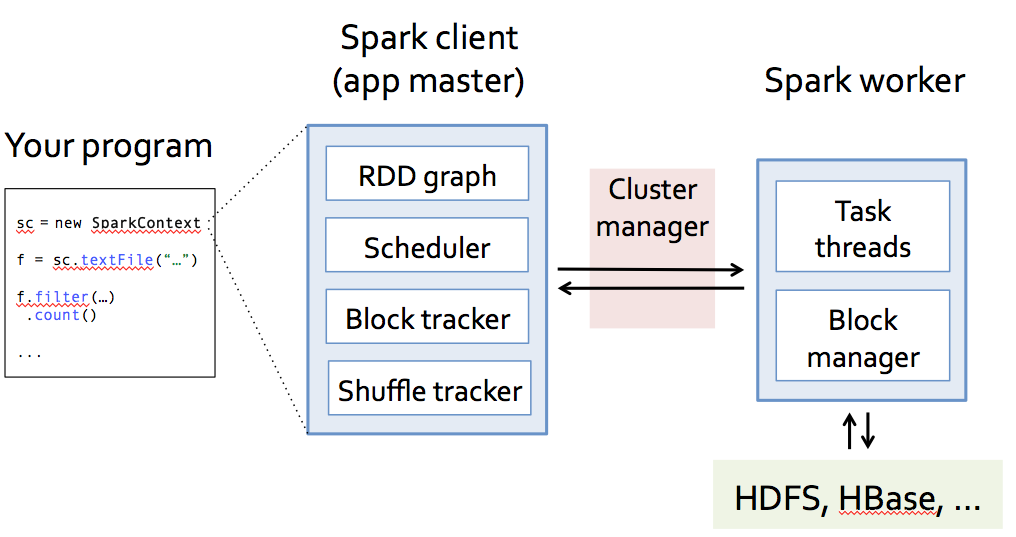
\includegraphics[scale=0.33]{./Figures/spark_components}
  \label{fig:spark_components}
\end{figure}
}

%%%%%%%%%%%%%%%%%%%%%%%%%%%%%%%%%%%%%%%%%%%%%%%%%%%%%%%%%%
\begin{frame}[fragile]
\frametitle{A Very Simple Job Example}
%%%%%%%%%%%%%%%%%%%%%%%%%%%%%%%%%%%%%%%%%%%%%%%%%%%%%%%%%%


\begin{lstlisting}
val sc = new SparkContext("spark://...", "MyJob", home, jars) 

val file = sc.textFile("hdfs://...") // This is an RDD

val errors = file.filter(_.contains("ERROR")) // This is an RDD

errors.cache()

errors.count() // This is an action
\end{lstlisting}

\end{frame}

%%%%%%%%%%%%%%%%%%%%%%%%%%%%%%%%%%%%%%%%%%%%%%%%%%%%%%%%%%
\begin{frame}
\frametitle{Spark Components: System-level View}
%%%%%%%%%%%%%%%%%%%%%%%%%%%%%%%%%%%%%%%%%%%%%%%%%%%%%%%%%%
	\begin{figure}[h]
	  \centering
	  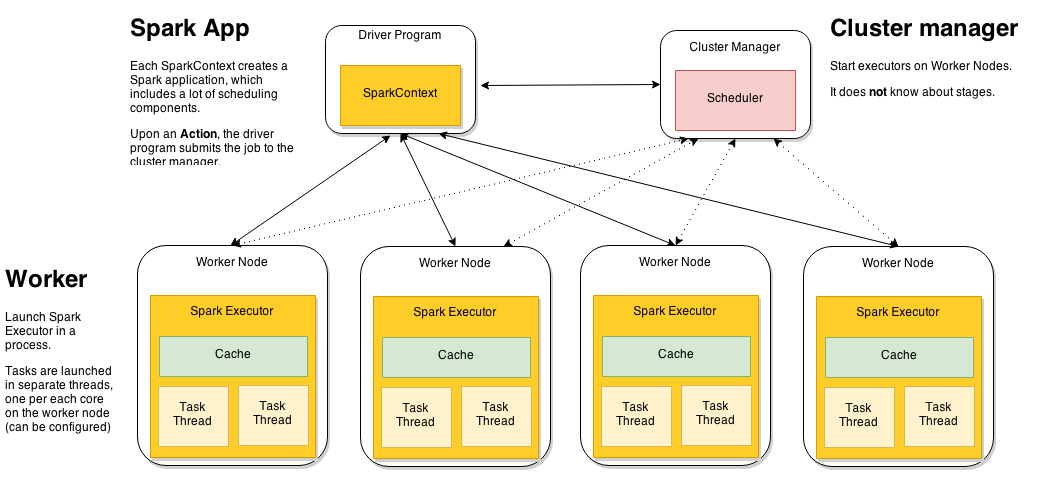
\includegraphics[scale=0.3]{./Figures/spark_system}
	  \label{fig:spark_components}
	\end{figure}
\end{frame}

%%%%%%%%%%%%%%%%%%%%%%%%%%%%%%%%%%%%%%%%%%%%%%%%%%%%%%%%%%
\frame {\frametitle{The RDD graph: dataset vs. partition views}
%%%%%%%%%%%%%%%%%%%%%%%%%%%%%%%%%%%%%%%%%%%%%%%%%%%%%%%%%%
% missing: what is an rdd? difference between RDD and partition?

\begin{columns}[c]
	\column{.5\textwidth}
		
			\begin{figure}[h]
			  \centering
			  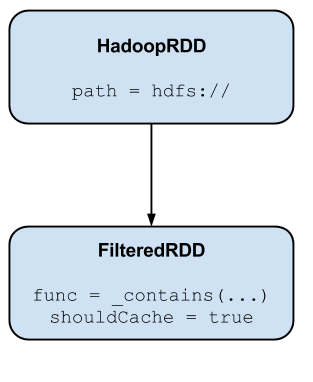
\includegraphics[scale=0.25]{./Figures/spark_rdd}
			  \label{fig:spark_components}
			\end{figure}
	
	\column{.5\textwidth}
		
			\begin{figure}[h]
			  \centering
			  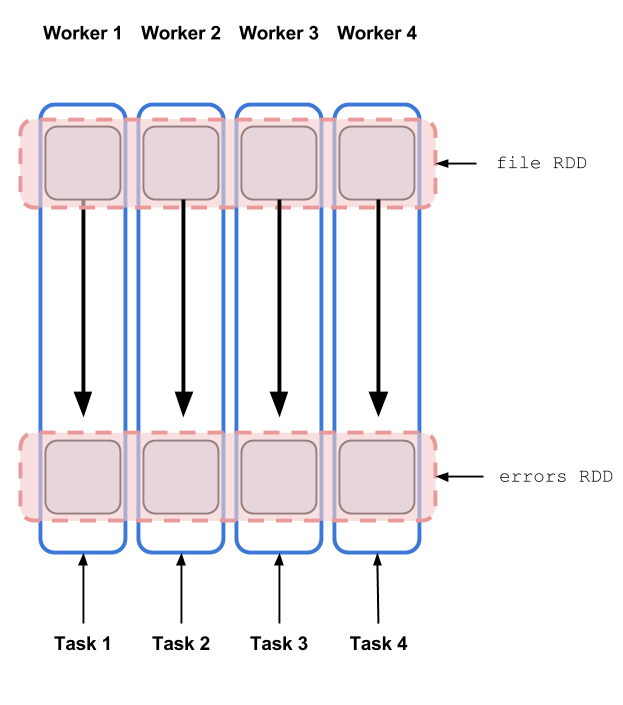
\includegraphics[scale=0.25]{./Figures/spark_partition}
			  \label{fig:spark_components}
			\end{figure}

\end{columns}
}

% %%%%%%%%%%%%%%%%%%%%%%%%%%%%%%%%%%%%%%%%%%%%%%%%%%%%%%%%%%
\frame {\frametitle{Data Locality}
% %%%%%%%%%%%%%%%%%%%%%%%%%%%%%%%%%%%%%%%%%%%%%%%%%%%%%%%%%%
\begin{itemize}
	\item {\bf Data locality principle}
	\begin{itemize}
		\item Same as for Hadoop MapReduce
		\item Avoid network I/O, workers should manage local data
	\end{itemize}

	\vspace{20pt}

	\item {\bf Data locality and caching}
	\begin{itemize}
		\item First run: data not in cache, so use HadoopRDD's locality prefs (from HDFS)
		\item Second run: FilteredRDD is in cache, so use its locations
		\item If something falls out of cache, go back to HDFS
	\end{itemize}
\end{itemize}
}



%%%%%%%%%%%%%%%%%%%%%%%%%%%%%%%%%%%%%%%%%%%%%%%%%%%%%%%%%%
\frame {\frametitle{Lifetime of a Job in Spark}
%%%%%%%%%%%%%%%%%%%%%%%%%%%%%%%%%%%%%%%%%%%%%%%%%%%%%%%%%%

\begin{columns}[t, onlytextwidth]
	\begin{column}[T]{.2\textwidth}
		\begin{center}
			{ \tiny \bf RDD Objects}
		\end{center}
		\begin{figure}[h]
			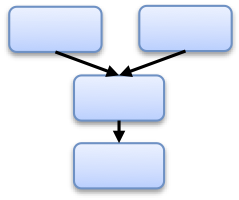
\includegraphics[scale=0.5]{./Figures/RDD_objects}
		\end{figure}

		\begin{colorblock}{blue}{lightblue}{ }
			{\tiny \texttt{
				rdd1.join(rdd2)\\
				\hspace{12pt} .groupBy(...)\\
				\hspace{12pt} .filter(...)\\
				}
			}
		\end{colorblock}

		\vspace{10pt}

		\begin{colorblock}{blue}{lightblue}{ }
			{\tiny \bf Build the operator DAG}
		\end{colorblock}
	\end{column}

	\begin{column}[T]{.2\textwidth}
		\begin{center}
			{ \tiny \bf DAG Scheduler}
		\end{center}			
		\begin{figure}[h]
			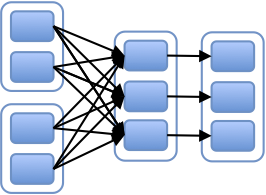
\includegraphics[scale=0.5]{./Figures/DAG_scheduler}
		\end{figure}

		\vspace{10pt}

		\begin{colorblock}{blue}{lightblue}{ }
			{\tiny \bf Split the DAG into \emph{stages} of \emph{tasks}}
		\end{colorblock}

		\vspace{10pt}

		\begin{colorblock}{blue}{lightblue}{ }
			{\tiny \bf Submit each stage and its tasks as ready}
		\end{colorblock}			
	\end{column}

	\begin{column}[T]{.2\textwidth}
		\begin{center}
			{ \tiny \bf Task Scheduler}
		\end{center}			

		\vspace{-20pt}

		\begin{figure}[h]
			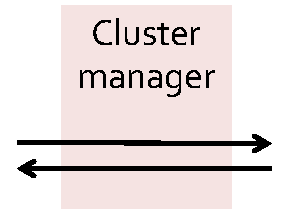
\includegraphics[scale=0.5]{./Figures/Task_scheduler}
		\end{figure}

		\vspace{10pt}

		\begin{colorblock}{blue}{lightblue}{ }
			{\tiny \bf Launch tasks via Master}
		\end{colorblock}

		\vspace{10pt}

		\begin{colorblock}{blue}{lightblue}{ }
			{\tiny \bf Retry failed and straggler tasks}
		\end{colorblock}			
	\end{column}

	\begin{column}[T]{.2\textwidth}
		\begin{center}
			{ \tiny \bf Worker}
		\end{center}			
		\begin{figure}[h]
			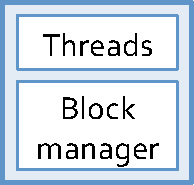
\includegraphics[scale=0.5]{./Figures/Worker}
		\end{figure}
		\vspace{10pt}

		\begin{colorblock}{blue}{lightblue}{ }
			{\tiny \bf Execute tasks}
		\end{colorblock}

		\vspace{10pt}

		\begin{colorblock}{blue}{lightblue}{ }
			{\tiny \bf Store and serve blocks}
		\end{colorblock}			
	\end{column}
\end{columns}
}

%%%%%%%%%%%%%%%%%%%%%%%%%%%%%%%%%%%%%%%%%%%%%%%%%%%%%%%%%%
\frame {\frametitle{What is an RDD}
%%%%%%%%%%%%%%%%%%%%%%%%%%%%%%%%%%%%%%%%%%%%%%%%%%%%%%%%%%
\begin{itemize}
	\item {\bf RDD are partitioned, locality aware, distributed collections}

	\vspace{20pt}

	\item {\bf RDD are data structures that:}
	\begin{itemize}
		\item Either point to a direct data source (e.g. HDFS)
		\item Apply some transformations to its parent RDD(s) to generate new data elements
	\end{itemize}

	\vspace{20pt}

	\item {\bf Computations on RDDs}
	\begin{itemize}
	 	\item Represented by \emph{lazily evaluated} lineage \emph{DAGs} composed by chained RDDs
	 \end{itemize} 
\end{itemize}
}

%%%%%%%%%%%%%%%%%%%%%%%%%%%%%%%%%%%%%%%%%%%%%%%%%%%%%%%%%%
\frame {\frametitle{RDD Abstraction}
%%%%%%%%%%%%%%%%%%%%%%%%%%%%%%%%%%%%%%%%%%%%%%%%%%%%%%%%%%
\begin{itemize}
	\item {\bf Overall objective}
	\begin{itemize}
		\item Support a wide array of operators (more than just \texttt{Map} and \texttt{Reduce})
		\item Allow arbitrary composition of such operators
	\end{itemize}

	\vspace{20pt}

	\item {\bf Simplify scheduling}
	\begin{itemize}
		\item Avoid to modify the scheduler for each operator
	\end{itemize}

	\vspace{20pt}

	\item[$\to$] The question is: \emph{How to capture dependencies in a general way?}
\end{itemize}
}

%%%%%%%%%%%%%%%%%%%%%%%%%%%%%%%%%%%%%%%%%%%%%%%%%%%%%%%%%%
\frame {\frametitle{RDD Interfaces}
%%%%%%%%%%%%%%%%%%%%%%%%%%%%%%%%%%%%%%%%%%%%%%%%%%%%%%%%%%
\begin{itemize}
	\item {\bf Set of partitions (``splits'')}
	\begin{itemize}
		\item Much like in Hadoop MapReduce, each RDD is associated to (input) partitions
	\end{itemize}

	\item {\bf List of dependencies on parent RDDs}
	\begin{itemize}
		\item This is completely new w.r.t. Hadoop MapReduce
	\end{itemize}

	\item {\bf Function to compute a partition given parents}
	\begin{itemize}
		\item This is actually the ``user-defined code'' we referred to when discussing about the \texttt{Mapper} and \texttt{Reducer} classes in Hadoop
	\end{itemize}

	\item {\bf Optional preferred locations}
	\begin{itemize}
		\item This is to enforce data locality
	\end{itemize}

	\item {\bf Optional partitioning info (Partitioner)}
	\begin{itemize}
		\item This really helps in some ``advanced'' scenarios in which you want to pay attention to the behavior of the shuffle mechanism
	\end{itemize}
\end{itemize}
}

%%%%%%%%%%%%%%%%%%%%%%%%%%%%%%%%%%%%%%%%%%%%%%%%%%%%%%%%%%
\frame {\frametitle{Hadoop RDD}
%%%%%%%%%%%%%%%%%%%%%%%%%%%%%%%%%%%%%%%%%%%%%%%%%%%%%%%%%%
\begin{itemize}
	\item {\color{mauve} partitions} = one per HDFS block

	\vspace{10pt}

	\item {\color{mauve} dependencies} = none

	\vspace{10pt}

	\item {\color{mauve} compute(partition)} = read corresponding block

	\vspace{10pt}

	\item {\color{mauve} preferredLocations(part)} = HDFS block location

	\vspace{10pt}

	\item {\color{mauve} partitioner} = none

\end{itemize}
}

%%%%%%%%%%%%%%%%%%%%%%%%%%%%%%%%%%%%%%%%%%%%%%%%%%%%%%%%%%
\frame {\frametitle{Filtered RDD}
%%%%%%%%%%%%%%%%%%%%%%%%%%%%%%%%%%%%%%%%%%%%%%%%%%%%%%%%%%
\begin{itemize}
	\item {\color{mauve} partitions} = same as parent RDD

	\vspace{10pt}

	\item {\color{mauve} dependencies} = \emph{one-to-one} on parent

	\vspace{10pt}

	\item {\color{mauve} compute(partition)} = compute parent and filter it

	\vspace{10pt}

	\item {\color{mauve} preferredLocations(part)} = none (\emph{ask parent})

	\vspace{10pt}

	\item {\color{mauve} partitioner} = none

\end{itemize}
}

%%%%%%%%%%%%%%%%%%%%%%%%%%%%%%%%%%%%%%%%%%%%%%%%%%%%%%%%%%
\frame {\frametitle{Joined RDD}
%%%%%%%%%%%%%%%%%%%%%%%%%%%%%%%%%%%%%%%%%%%%%%%%%%%%%%%%%%
\begin{itemize}
	\item {\color{mauve} partitions} = one per reduce task

	\vspace{10pt}

	\item {\color{mauve} dependencies} = \emph{shuffle} on \emph{each} parent

	\vspace{10pt}

	\item {\color{mauve} compute(partition)} = read and join shuffled data

	\vspace{10pt}

	\item {\color{mauve} preferredLocations(part)} = none 

	\vspace{10pt}

	\item {\color{mauve} partitioner} = HashPartitioner(numTask)\footnote{Spark knows this data is hashed.}

\end{itemize}
}

%%%%%%%%%%%%%%%%%%%%%%%%%%%%%%%%%%%%%%%%%%%%%%%%%%%%%%%%%%
\frame {\frametitle{Dependency Types}
%%%%%%%%%%%%%%%%%%%%%%%%%%%%%%%%%%%%%%%%%%%%%%%%%%%%%%%%%%
\begin{columns}[t, onlytextwidth]
	\begin{column}[T]{.4\textwidth}
		\begin{center}
			{ \tiny \bf Narrow dependencies}
		\end{center}
		\begin{figure}[h]
			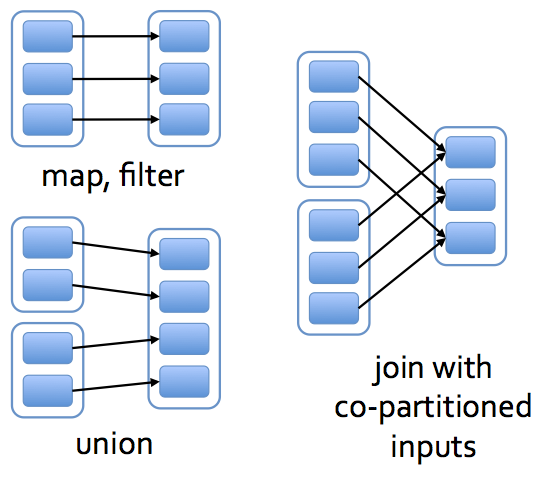
\includegraphics[scale=0.3]{./Figures/narrow_deps}
		\end{figure}
	\end{column}

	\begin{column}[T]{.4\textwidth}
		\begin{center}
			{ \tiny \bf Wide dependencies}
		\end{center}
		\begin{figure}[h]
			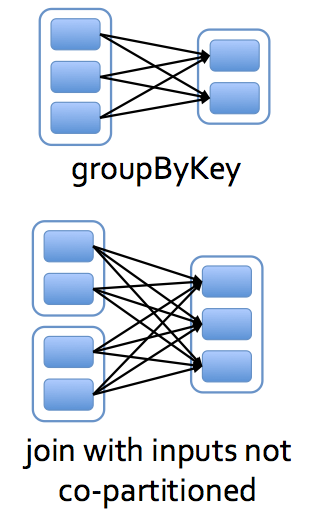
\includegraphics[scale=0.3]{./Figures/wide_deps}
		\end{figure}
	\end{column}
\end{columns}
}

%%%%%%%%%%%%%%%%%%%%%%%%%%%%%%%%%%%%%%%%%%%%%%%%%%%%%%%%%%
\frame {\frametitle{RDD Code Snippet}
%%%%%%%%%%%%%%%%%%%%%%%%%%%%%%%%%%%%%%%%%%%%%%%%%%%%%%%%%%
	\begin{figure}[h]
	\center
		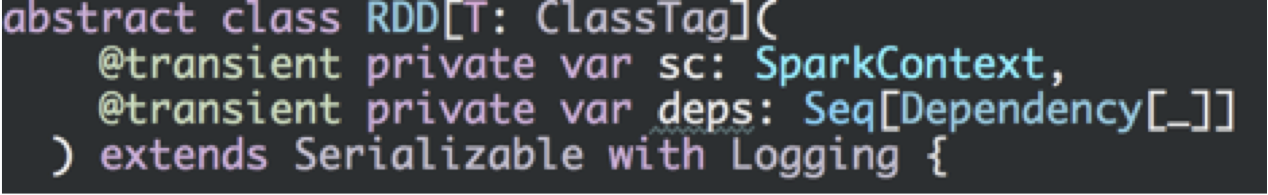
\includegraphics[scale=0.5]{./Figures/rdd_snippet}
	\end{figure}


	\begin{itemize}
		\item {\bf SparkContext}
		\begin{itemize}
			\item This is the main entity responsible for setting up a job
			\item Contains SparkConfig, Scheduler, entry point of running jobs (runJobs)
		\end{itemize}

		\vspace{15pt}

		\item {\bf Dependencies}
		\begin{itemize}
			\item Input RDD(s)
		\end{itemize}
	\end{itemize}

	\begin{colorblock}{blue}{lightblue}{}
	{\bf M. Zaharia}, M. Chowdhury, T. Das, A. Dave, J. Ma, M. McCauley, M.J. Franklin, S. Shenker, I. Stoica. \emph{Resilient Distributed Datasets: A Fault-Tolerant Abstraction for In-Memory Cluster Computing}, {\bf NSDI}, 2012		
	\end{colorblock}			
}

%%%%%%%%%%%%%%%%%%%%%%%%%%%%%%%%%%%%%%%%%%%%%%%%%%%%%%%%%%
\frame {\frametitle{RDD.map operation Snippet}
%%%%%%%%%%%%%%%%%%%%%%%%%%%%%%%%%%%%%%%%%%%%%%%%%%%%%%%%%%
	\begin{itemize}
		\item {\bf Map: RDD[T] $\to$ RDD[U]}
	\end{itemize}

	\begin{figure}[h]
	\center
		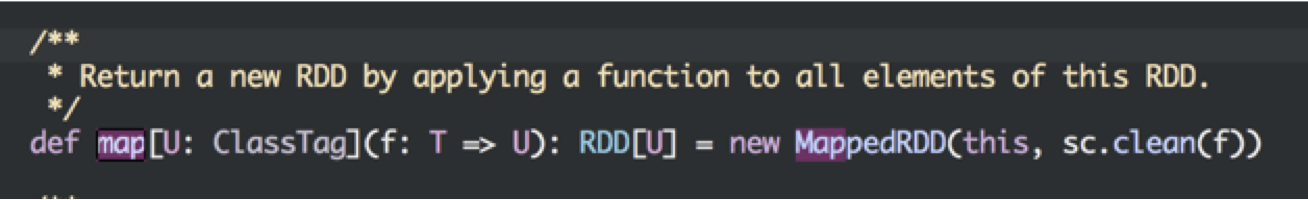
\includegraphics[scale=0.5]{./Figures/rddmap_snippet}
	\end{figure}

	\begin{itemize}
		\item {\bf MappedRDD}
		\begin{itemize}
			\item For each element in a partition, apply function $f$
		\end{itemize}
	\end{itemize}

	\begin{figure}[h]
	\center
		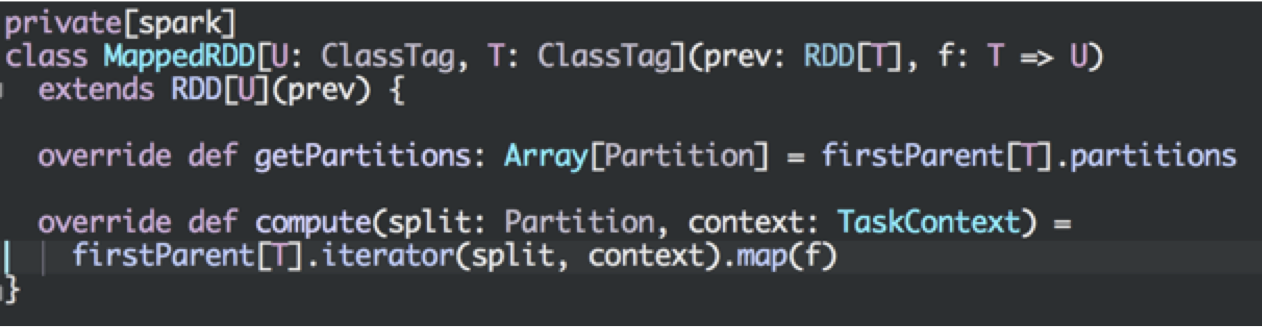
\includegraphics[scale=0.5]{./Figures/mappedrdd_snippet}
	\end{figure}

}

%%%%%%%%%%%%%%%%%%%%%%%%%%%%%%%%%%%%%%%%%%%%%%%%%%%%%%%%%%
\frame {\frametitle{RDD Iterator Code Snipped}
%%%%%%%%%%%%%%%%%%%%%%%%%%%%%%%%%%%%%%%%%%%%%%%%%%%%%%%%%%
\begin{itemize}
	\item {\bf Method to go through an RDD and apply function $f$}
	\begin{itemize}
		\item First, check local cache
		\item If not found, compute the RDD
	\end{itemize}
\end{itemize}

	\begin{figure}[h]
	\center
		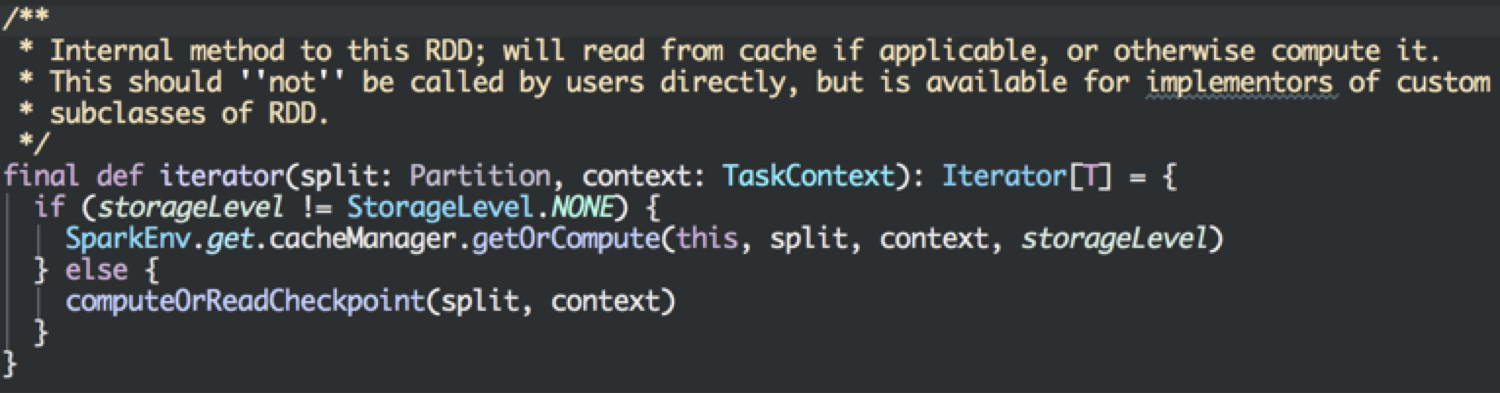
\includegraphics[scale=0.45]{./Figures/iterator_snippet}
	\end{figure}


\begin{itemize}
	\item {\bf Storage Levels}
	\begin{itemize}
		\item Disk
		\item Memory
		\item Off Heap (e.g. external memory stores like Tachyon)
		\item De-serialized
	\end{itemize}
\end{itemize}

}

%%%%%%%%%%%%%%%%%%%%%%%%%%%%%%%%%%%%%%%%%%%%%%%%%%%%%%%%%%
\frame {\frametitle{Making RDD from local collections}
%%%%%%%%%%%%%%%%%%%%%%%%%%%%%%%%%%%%%%%%%%%%%%%%%%%%%%%%%%
	\begin{itemize}
		\item {\bf Convert a local (on the driver) Seq[T] into RDD[T]}
	\end{itemize}

	\begin{figure}[h]
	\center
		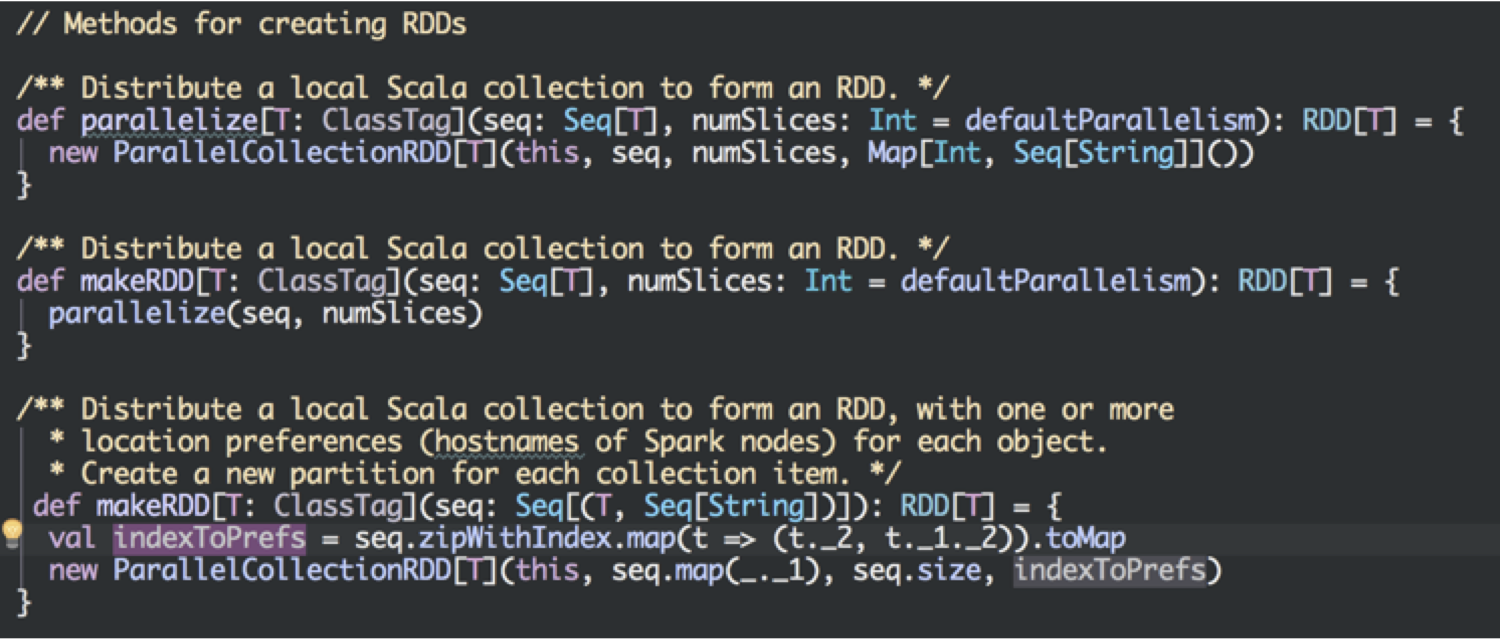
\includegraphics[scale=0.45]{./Figures/parallelize_snippet}
	\end{figure}


}

%%%%%%%%%%%%%%%%%%%%%%%%%%%%%%%%%%%%%%%%%%%%%%%%%%%%%%%%%%
\frame {\frametitle{Hadoop RDD Code Snippet}
%%%%%%%%%%%%%%%%%%%%%%%%%%%%%%%%%%%%%%%%%%%%%%%%%%%%%%%%%%
\begin{itemize}
	\item {\bf Reading HDFS data as <key, value> records}
\end{itemize}

\begin{figure}[h]
	\center
		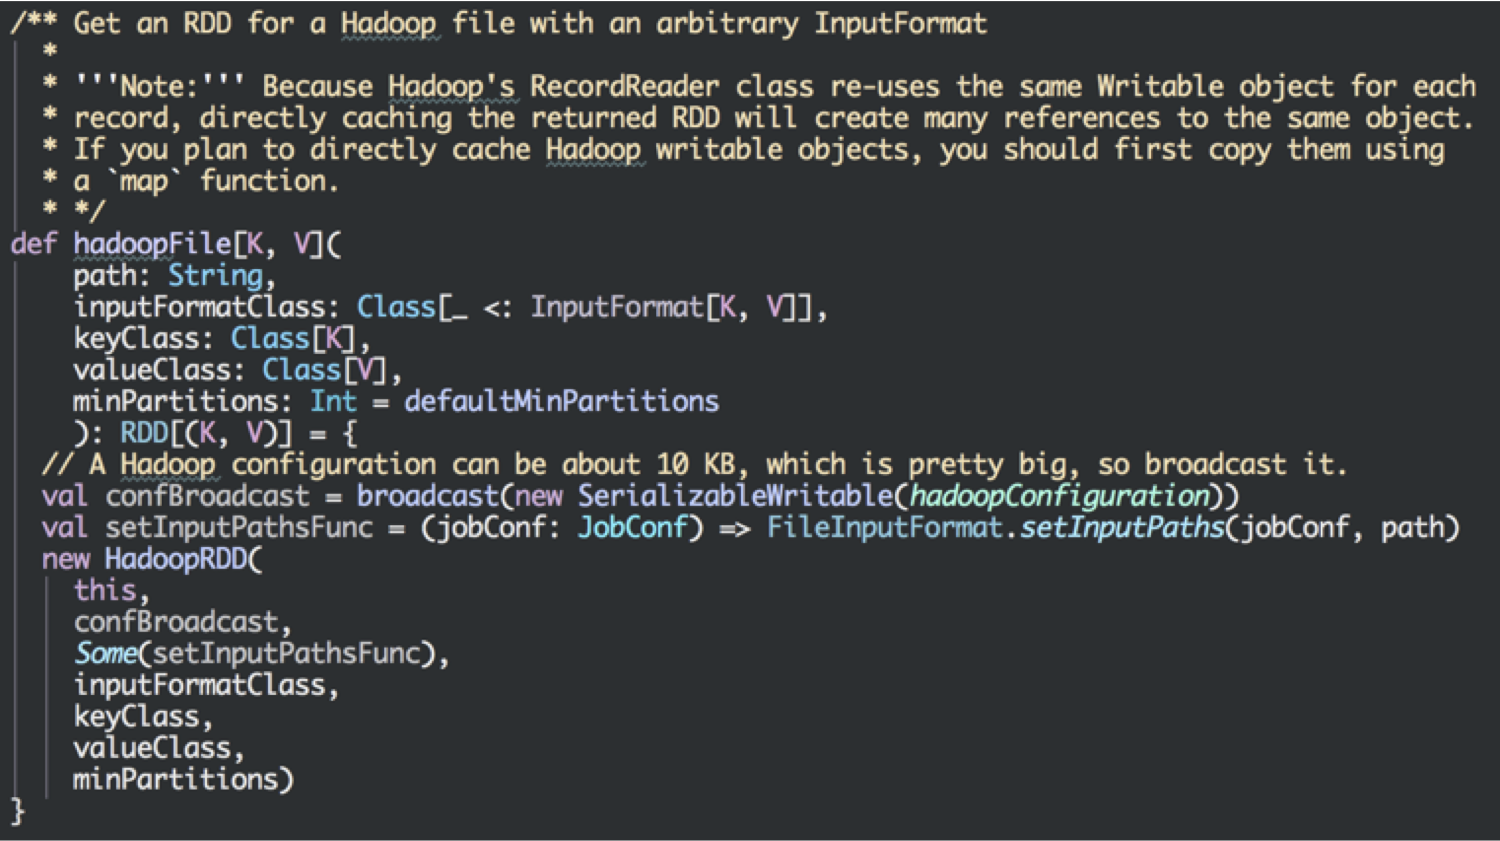
\includegraphics[scale=0.45]{./Figures/HadoopRDD_snippet}
\end{figure}
}


%%%%%%%%%%%%%%%%%%%%%%%%%%%%%%%%%%%%%%%%%%%%%%%%%%%%%%%%%%

%%%%%%%%%%%%%%%%%%%%%%%%%%%%%%%%%%%%%%%%%%%%%%%%%%%%%%%%%%
\section{Spark Deployments}

\begin{frame}
 \begin{colorblock}{blue}{lightblue}{ }
  \begin{center}
    \Huge \textbf{\texttt{Spark Deployments}}
  \end{center}
  \end{colorblock}
\end{frame}

%%%%%%%%%%%%%%%%%%%%%%%%%%%%%%%%%%%%%%%%%%%%%%%%%%%%%%%%%%
\begin{frame}
\frametitle{Spark Components: System-level View}
%%%%%%%%%%%%%%%%%%%%%%%%%%%%%%%%%%%%%%%%%%%%%%%%%%%%%%%%%%
	\begin{figure}[h]
	  \centering
	  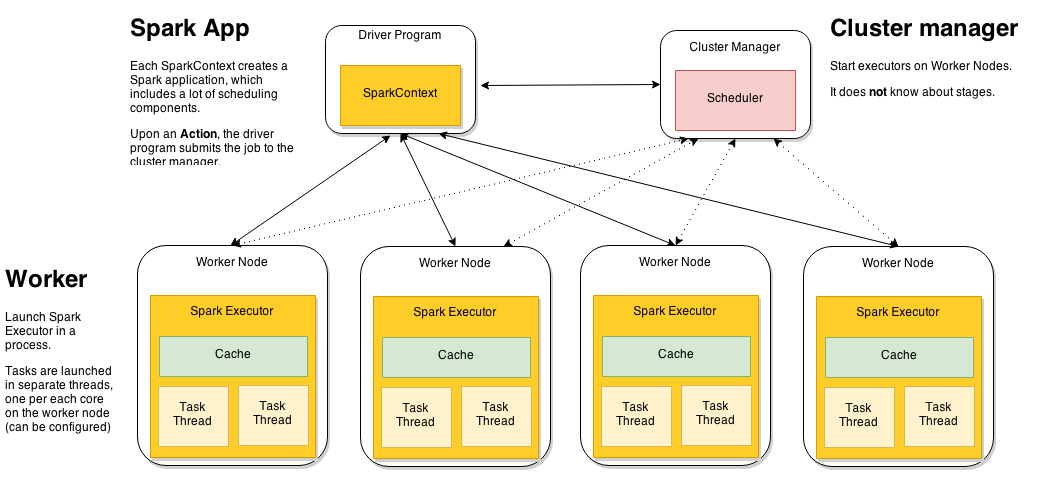
\includegraphics[scale=0.33]{./Figures/spark_system}
	  \label{fig:spark_components}
	\end{figure}
\end{frame}

%%%%%%%%%%%%%%%%%%%%%%%%%%%%%%%%%%%%%%%%%%%%%%%%%%%%%%%%%%
\begin{frame}
\frametitle{Spark Deployment Modes}
%%%%%%%%%%%%%%%%%%%%%%%%%%%%%%%%%%%%%%%%%%%%%%%%%%%%%%%%%%
\begin{itemize}
	\item {\bf The Spark Framework can adopt several cluster managers}
	\begin{itemize}
		\item \emph{Local Mode}
		\item \emph{Standalone mode}
		\item \emph{Apache Mesos}
		\item \emph{Hadoop YARN}
	\end{itemize}

	\vspace{20pt}

	\item {\bf General ``workflow''}
	\begin{itemize}
		\item Spark application creates \texttt{SparkContext}, which initializes the \texttt{DriverProgram}
		\item Registers to the \texttt{ClusterManager}
		\item Ask resources to allocate Executors
		\item Schedule Task execution
	\end{itemize}
\end{itemize}
\end{frame}

%%%%%%%%%%%%%%%%%%%%%%%%%%%%%%%%%%%%%%%%%%%%%%%%%%%%%%%%%%
\begin{frame}
\frametitle{Worker Nodes and Executors}
%%%%%%%%%%%%%%%%%%%%%%%%%%%%%%%%%%%%%%%%%%%%%%%%%%%%%%%%%%
\begin{figure}[h]
  \centering
  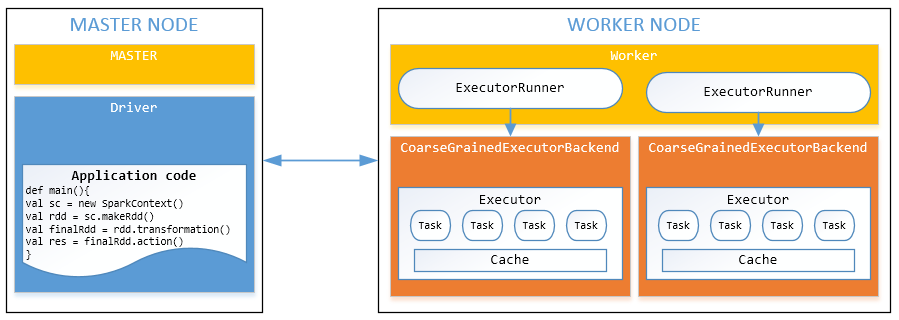
\includegraphics[scale=0.35]{./Figures/spark_worker_executor}
  \label{fig:spark_shuffle_sort}
\end{figure}

\begin{itemize}
	\item {\bf Worker nodes are machines that run executors}
	\begin{itemize}
		\item Host one or multiple \texttt{Workers}
		\item One JVM (= 1 UNIX process) per \texttt{Worker}
		\item Each \texttt{Worker} can spawn one or more \texttt{Executors}
	\end{itemize}

	\item {\bf Executors run tasks}
	\begin{itemize}
		\item Run in child JVM (= 1 UNIX process)
		\item Execute one or more task using threads in a \texttt{ThreadPool}
	\end{itemize}
\end{itemize}
\end{frame}

%%%%%%%%%%%%%%%%%%%%%%%%%%%%%%%%%%%%%%%%%%%%%%%%%%%%%%%%%%
\begin{frame}
\frametitle{Comparison to Hadoop MapReduce}
%%%%%%%%%%%%%%%%%%%%%%%%%%%%%%%%%%%%%%%%%%%%%%%%%%%%%%%%%%
\begin{columns}[t, onlytextwidth]
	\column[T]{.5\textwidth}
	{\bf Hadoop MapReduce}
	\begin{itemize}
		\item One Task per UNIX process (JVM), more if JVM reuse
		\item \texttt{MultiThreadedMapper}, advanced feature to have threads in Map Tasks
		\item[$\to$] {\bf Short-lived} Executor, with one {\bf large Task}
	\end{itemize}

	
	\column[T]{.5\textwidth}
	{\bf Spark}		
	\begin{itemize}
		\item Tasks run in one or more Threads, within a single UNIX process (JVM)
		\item Executor process statically allocated to worker, even with no threads
		\item[$\to$] {\bf Long-lived} Executor, with many {\bf small Tasks}
	\end{itemize}

\end{columns}

\end{frame}

%%%%%%%%%%%%%%%%%%%%%%%%%%%%%%%%%%%%%%%%%%%%%%%%%%%%%%%%%%
\begin{frame}
\frametitle{Benefits of the Spark Architecture}
%%%%%%%%%%%%%%%%%%%%%%%%%%%%%%%%%%%%%%%%%%%%%%%%%%%%%%%%%%
\begin{itemize}
	\item {\bf Isolation}
	\begin{itemize}
		\item Applications are completely isolated
		\item Task scheduling \emph{per application}
	\end{itemize}

	\item {\bf Low-overhead}
	\begin{itemize}
		\item Task setup cost is that of spawning a thread, not a process
		\item 10-100 times faster
		\item {\color{red} Small tasks $\to$ mitigate effects of data skew}
	\end{itemize}

	\item {\bf Sharing data}
	\begin{itemize}
		\item Applications cannot share data in memory natively
		\item Use an external storage service like Tachyon
	\end{itemize}

	\item {\bf Resource allocation}
	\begin{itemize}
		\item Static process provisioning for executors, even without active tasks
		\item Dynamic provisioning under development
	\end{itemize}
\end{itemize}
\end{frame}

%%%%%%%%%%%%%%%%%%%%%%%%%%%%%%%%%%%%%%%%%%%%%%%%%%%%%%%%%%


%%%%%%%%%%%%%%%%%%%%%%%%%%%%%%%%%%%%%%%%%%%%%%%%%%%%%%%%%%
\section{Resilient Distributed Datasets}

\begin{frame}
 \begin{colorblock}{blue}{lightblue}{ }
  \begin{center}
    \Huge \textbf{\texttt{Resilient Distributed Datasets}}
  \end{center}
  \end{colorblock}

  \vspace{20pt}

  \begin{colorblock}{blue}{lightblue}{}
  {\bf M. Zaharia}, M. Chowdhury, T. Das, A. Dave, J. Ma, M. McCauley, M.J. Franklin, S. Shenker, I. Stoica.\\
  \emph{Resilient Distributed Datasets: A Fault-Tolerant Abstraction for In-Memory Cluster Computing},\\
  {\bf USENIX Symposium on Networked Systems Design and Implementation}, 2012    
  \end{colorblock}      


\end{frame}

%%%%%%%%%%%%%%%%%%%%%%%%%%%%%%%%%%%%%%%%%%%%%%%%%%%%%%%%%%
\frame {\frametitle{What is an RDD}
%%%%%%%%%%%%%%%%%%%%%%%%%%%%%%%%%%%%%%%%%%%%%%%%%%%%%%%%%%
\begin{itemize}
	\item {\bf RDD are partitioned, locality aware, distributed collections}
	\begin{itemize}
		\item RDD are \emph{immutable}
	\end{itemize}

	\vspace{20pt}

	\item {\bf RDD are data structures that:}
	\begin{itemize}
		\item Either point to a direct data source (e.g. HDFS)
		\item Apply some transformations to its parent RDD(s) to generate new data elements
	\end{itemize}

	\vspace{20pt}

	\item {\bf Computations on RDDs}
	\begin{itemize}
	 	\item Represented by \emph{lazily evaluated} lineage \emph{DAGs} composed by chained RDDs
	 \end{itemize} 
\end{itemize}
}

%%%%%%%%%%%%%%%%%%%%%%%%%%%%%%%%%%%%%%%%%%%%%%%%%%%%%%%%%%
\frame {\frametitle{RDD Abstraction}
%%%%%%%%%%%%%%%%%%%%%%%%%%%%%%%%%%%%%%%%%%%%%%%%%%%%%%%%%%
\begin{itemize}
	\item {\bf Overall objective}
	\begin{itemize}
		\item Support a wide array of operators (more than just \texttt{Map} and \texttt{Reduce})
		\item Allow arbitrary composition of such operators
	\end{itemize}

	\vspace{20pt}

	\item {\bf Simplify scheduling}
	\begin{itemize}
		\item Avoid to modify the scheduler for each operator
	\end{itemize}

	\vspace{20pt}

	\item[$\to$] The question is: \emph{How to capture dependencies in a general way?}
\end{itemize}
}

%%%%%%%%%%%%%%%%%%%%%%%%%%%%%%%%%%%%%%%%%%%%%%%%%%%%%%%%%%
\frame {\frametitle{RDD Interfaces}
%%%%%%%%%%%%%%%%%%%%%%%%%%%%%%%%%%%%%%%%%%%%%%%%%%%%%%%%%%
\begin{itemize}
	\item {\bf Set of partitions (``splits'')}
	\begin{itemize}
		\item Much like in Hadoop MapReduce, each RDD is associated to (input) partitions
	\end{itemize}

	\item {\bf List of dependencies on parent RDDs}
	\begin{itemize}
		\item This is completely new w.r.t. Hadoop MapReduce
	\end{itemize}

	\item {\bf Function to compute a partition given parents}
	\begin{itemize}
		\item This is actually the ``user-defined code'' we referred to when discussing about the \texttt{Mapper} and \texttt{Reducer} classes in Hadoop
	\end{itemize}

	\item {\bf Optional preferred locations}
	\begin{itemize}
		\item This is to enforce data locality
	\end{itemize}

	\item {\bf Optional partitioning info (Partitioner)}
	\begin{itemize}
		\item This really helps in some ``advanced'' scenarios in which you want to pay attention to the behavior of the shuffle mechanism
	\end{itemize}
\end{itemize}
}

%%%%%%%%%%%%%%%%%%%%%%%%%%%%%%%%%%%%%%%%%%%%%%%%%%%%%%%%%%
\frame {\frametitle{Hadoop RDD}
%%%%%%%%%%%%%%%%%%%%%%%%%%%%%%%%%%%%%%%%%%%%%%%%%%%%%%%%%%
\begin{itemize}
	\item {\color{mauve} partitions} = one per HDFS block

	\vspace{10pt}

	\item {\color{mauve} dependencies} = none

	\vspace{10pt}

	\item {\color{mauve} compute(partition)} = read corresponding block

	\vspace{10pt}

	\item {\color{mauve} preferredLocations(part)} = HDFS block location

	\vspace{10pt}

	\item {\color{mauve} partitioner} = none

\end{itemize}
}

%%%%%%%%%%%%%%%%%%%%%%%%%%%%%%%%%%%%%%%%%%%%%%%%%%%%%%%%%%
\frame {\frametitle{Filtered RDD}
%%%%%%%%%%%%%%%%%%%%%%%%%%%%%%%%%%%%%%%%%%%%%%%%%%%%%%%%%%
\begin{itemize}
	\item {\color{mauve} partitions} = same as parent RDD

	\vspace{10pt}

	\item {\color{mauve} dependencies} = \emph{one-to-one} on parent

	\vspace{10pt}

	\item {\color{mauve} compute(partition)} = compute parent and filter it

	\vspace{10pt}

	\item {\color{mauve} preferredLocations(part)} = none (\emph{ask parent})

	\vspace{10pt}

	\item {\color{mauve} partitioner} = none

\end{itemize}
}

%%%%%%%%%%%%%%%%%%%%%%%%%%%%%%%%%%%%%%%%%%%%%%%%%%%%%%%%%%
\frame {\frametitle{Joined RDD}
%%%%%%%%%%%%%%%%%%%%%%%%%%%%%%%%%%%%%%%%%%%%%%%%%%%%%%%%%%
\begin{itemize}
	\item {\color{mauve} partitions} = one per reduce task

	\vspace{10pt}

	\item {\color{mauve} dependencies} = \emph{shuffle} on \emph{each} parent

	\vspace{10pt}

	\item {\color{mauve} compute(partition)} = read and join shuffled data

	\vspace{10pt}

	\item {\color{mauve} preferredLocations(part)} = none 

	\vspace{10pt}

	\item {\color{mauve} partitioner} = HashPartitioner(numTask)\footnote{Spark knows this data is hashed.}

\end{itemize}
}

%%%%%%%%%%%%%%%%%%%%%%%%%%%%%%%%%%%%%%%%%%%%%%%%%%%%%%%%%%
\frame {\frametitle{Dependency Types (1)}
%%%%%%%%%%%%%%%%%%%%%%%%%%%%%%%%%%%%%%%%%%%%%%%%%%%%%%%%%%
\begin{columns}[t, onlytextwidth]
	\begin{column}[T]{.4\textwidth}
		\begin{center}
			{ \tiny \bf Narrow dependencies}
		\end{center}
		\begin{figure}[h]
			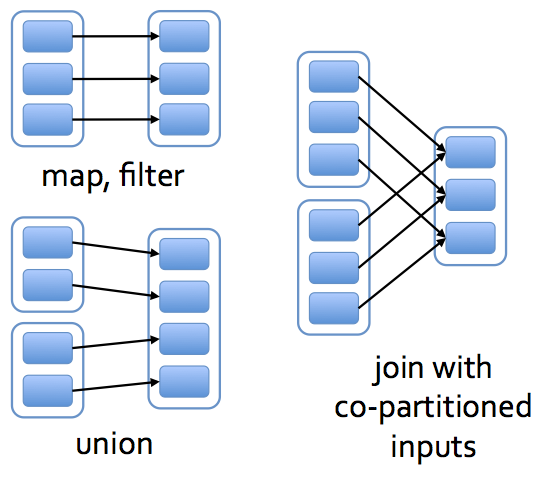
\includegraphics[scale=0.3]{./Figures/narrow_deps}
		\end{figure}
	\end{column}

	\begin{column}[T]{.4\textwidth}
		\begin{center}
			{ \tiny \bf Wide dependencies}
		\end{center}
		\begin{figure}[h]
			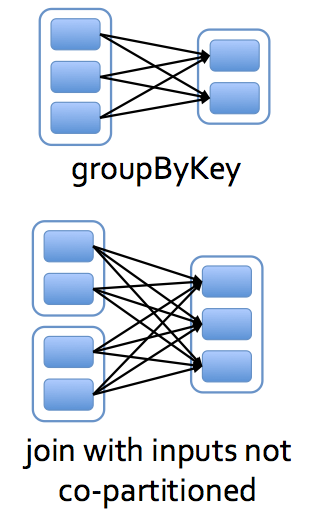
\includegraphics[scale=0.3]{./Figures/wide_deps}
		\end{figure}
	\end{column}
\end{columns}
}

%%%%%%%%%%%%%%%%%%%%%%%%%%%%%%%%%%%%%%%%%%%%%%%%%%%%%%%%%%
\frame {\frametitle{Dependency Types (2)}
%%%%%%%%%%%%%%%%%%%%%%%%%%%%%%%%%%%%%%%%%%%%%%%%%%%%%%%%%%
\begin{itemize}
	\item {\bf Narrow dependencies}
	\begin{itemize}
		\item Each partition of the parent RDD is used by at most one partition of the child RDD
		\item Task can be executed locally and we don't have to shuffle. (Eg: \texttt{map}, \texttt{flatMap}, \texttt{filter}, \texttt{sample})
	\end{itemize}

	\vspace{20pt}

	\item {\bf Wide Dependencies}
	\begin{itemize}
		\item Multiple child partitions may depend on one partition of the parent RDD 
		\item This means we have to shuffle data \textbf{unless the parents are hash-partitioned} (Eg: \texttt{sortByKey}, \texttt{reduceByKey}, \texttt{groupByKey}, \texttt{cogroupByKey}, \texttt{join}, \texttt{cartesian})
	\end{itemize}
\end{itemize}
}

%%%%%%%%%%%%%%%%%%%%%%%%%%%%%%%%%%%%%%%%%%%%%%%%%%%%%%%%%%
\frame {\frametitle{Dependency Types: Optimizations}
%%%%%%%%%%%%%%%%%%%%%%%%%%%%%%%%%%%%%%%%%%%%%%%%%%%%%%%%%%
\begin{itemize}
	\item {\bf Benefits of Lazy evaluation}
	\begin{itemize}
		\item The DAG Scheduler optimizes \emph{Stages} and \emph{Tasks} before submitting them to the Task Scheduler
		\item \textbf{Piplining} narrow dependencies within a Stage
		\item \textbf{Join plan selection} based on partitioning
		\item \textbf{Cache reuse}
	\end{itemize}
\end{itemize}

\begin{figure}[h]
	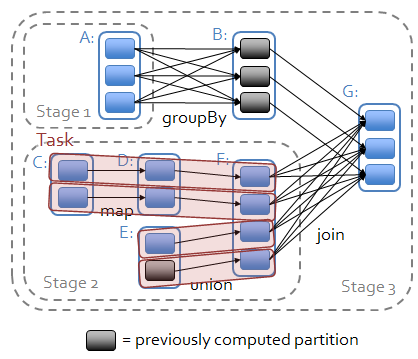
\includegraphics[scale=0.5]{./Figures/deps_optimization}
\end{figure}

}


%%%%%%%%%%%%%%%%%%%%%%%%%%%%%%%%%%%%%%%%%%%%%%%%%%%%%%%%%%
\frame {\frametitle{Operations on RDDs: Transformations}
%%%%%%%%%%%%%%%%%%%%%%%%%%%%%%%%%%%%%%%%%%%%%%%%%%%%%%%%%%
\begin{itemize}
	\item {\bf Transformations}
	\begin{itemize}
		\item Set of operations on a RDD that define how they should be transformed
		\item As in relational algebra, the application of a transformation to an RDD yields a new RDD (because RDD are \emph{immutable})
		\item Transformations are lazily evaluated, which allow for optimizations to take place before execution
	\end{itemize}

	\vspace{10pt}

	\item {\bf Examples} (not exhaustive)
	\begin{itemize}
		\item \texttt{map(func)}, \texttt{flatMap(func)}, \texttt{filter(func)}
		\item \texttt{grouByKey()}
		\item \texttt{reduceByKey(func)}, \texttt{mapValues(func)}, \texttt{distinct()}, \texttt{sortByKey(func)}
		\item \texttt{join(other)}, \texttt{union(other)}
		\item \texttt{sample()}
	\end{itemize}

\end{itemize}

}

%%%%%%%%%%%%%%%%%%%%%%%%%%%%%%%%%%%%%%%%%%%%%%%%%%%%%%%%%%
\frame {\frametitle{Operations on RDDs: Actions}
%%%%%%%%%%%%%%%%%%%%%%%%%%%%%%%%%%%%%%%%%%%%%%%%%%%%%%%%%%
\begin{itemize}
	\item {\bf Actions}
	\begin{itemize}
		\item Apply transformation chains on RDDs, eventually performing some additional operations (e.g., counting)
		\item Some actions only store data to an external data source (e.g. HDFS), others fetch data from the RDD (and its transformation chain) upon which the action is applied, and convey it to the driver
	\end{itemize}

	\vspace{20pt}

	\item {\bf Examples} (not exhaustive)
	\begin{itemize}
		\item \texttt{reduce(func)}
		\item \texttt{collect()}, \texttt{first()}, \texttt{take()}, \texttt{foreach(func)}
		\item \texttt{count()}, \texttt{countByKey()}
		\item \texttt{saveAsTextFile()}
	\end{itemize}

\end{itemize}
}

%%%%%%%%%%%%%%%%%%%%%%%%%%%%%%%%%%%%%%%%%%%%%%%%%%%%%%%%%%
\frame {\frametitle{Operations on RDDs: Final Notes}
%%%%%%%%%%%%%%%%%%%%%%%%%%%%%%%%%%%%%%%%%%%%%%%%%%%%%%%%%%
\begin{itemize}

	\item {\bf Look at return types!}
	\begin{itemize}
		\item Return type: RDD $\to$ transformation
		\item Return type: built-in scala/java types such as \texttt{int}, \texttt{long}, \texttt{List<Object>}, \texttt{Array<Object>} $\to$ action
	\end{itemize}

	\vspace{10pt}

	\item {\bf Caching is a transformation}
	\begin{itemize}
		\item Hints to keep RDD in memory after its first evaluation
	\end{itemize}

	\vspace{10pt}

	\item {\bf Transformations depend on RDD ``flavor''}
	\begin{itemize}
		\item \texttt{PairRDD}
		\item \texttt{SchemaRDD}
	\end{itemize}

\end{itemize}
}


%%%%%%%%%%%%%%%%%%%%%%%%%%%%%%%%%%%%%%%%%%%%%%%%%%%%%%%%%%
\frame {\frametitle{RDD Code Snippet}
%%%%%%%%%%%%%%%%%%%%%%%%%%%%%%%%%%%%%%%%%%%%%%%%%%%%%%%%%%
	\begin{figure}[h]
	\center
		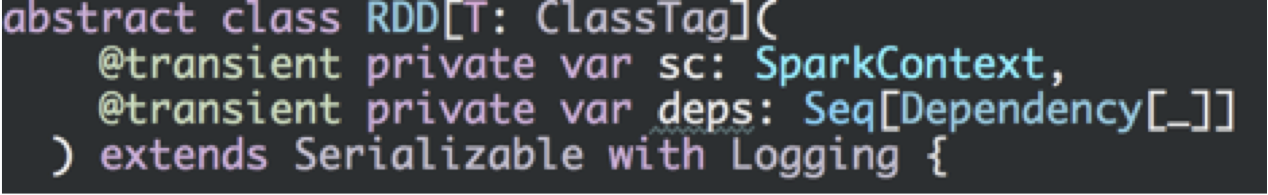
\includegraphics[scale=0.5]{./Figures/rdd_snippet}
	\end{figure}


	\begin{itemize}
		\item {\bf SparkContext}
		\begin{itemize}
			\item This is the main entity responsible for setting up a job
			\item Contains SparkConfig, Scheduler, entry point of running jobs (runJobs)
		\end{itemize}

		\vspace{15pt}

		\item {\bf Dependencies}
		\begin{itemize}
			\item Input RDD(s)
		\end{itemize}
	\end{itemize}
}

%%%%%%%%%%%%%%%%%%%%%%%%%%%%%%%%%%%%%%%%%%%%%%%%%%%%%%%%%%
\frame {\frametitle{RDD.map operation Snippet}
%%%%%%%%%%%%%%%%%%%%%%%%%%%%%%%%%%%%%%%%%%%%%%%%%%%%%%%%%%
	\begin{itemize}
		\item {\bf Map: RDD[T] $\to$ RDD[U]}
	\end{itemize}

	\begin{figure}[h]
	\center
		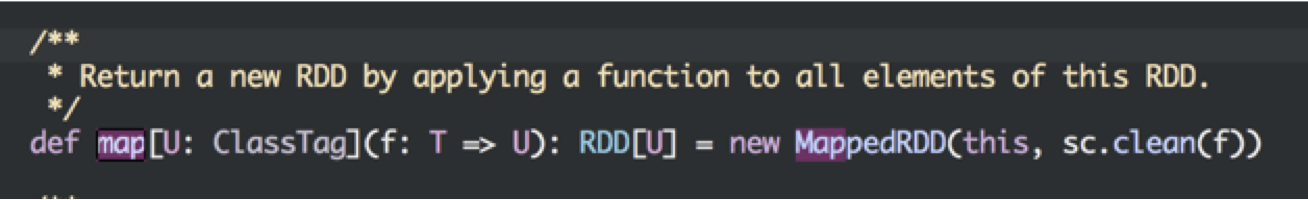
\includegraphics[scale=0.5]{./Figures/rddmap_snippet}
	\end{figure}

	\begin{itemize}
		\item {\bf MappedRDD}
		\begin{itemize}
			\item For each element in a partition, apply function $f$
		\end{itemize}
	\end{itemize}

	\begin{figure}[h]
	\center
		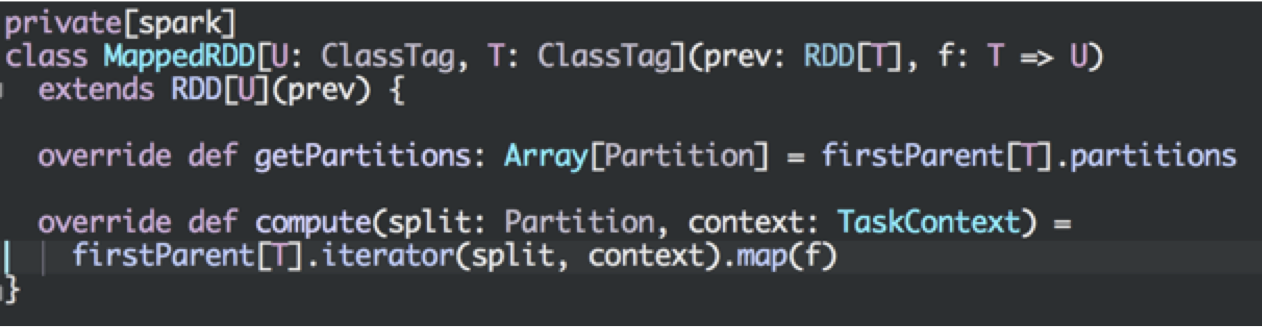
\includegraphics[scale=0.5]{./Figures/mappedrdd_snippet}
	\end{figure}

}

%%%%%%%%%%%%%%%%%%%%%%%%%%%%%%%%%%%%%%%%%%%%%%%%%%%%%%%%%%
\frame {\frametitle{RDD Iterator Code Snipped}
%%%%%%%%%%%%%%%%%%%%%%%%%%%%%%%%%%%%%%%%%%%%%%%%%%%%%%%%%%
\begin{itemize}
	\item {\bf Method to go through an RDD and apply function $f$}
	\begin{itemize}
		\item First, check local cache
		\item If not found, compute the RDD
	\end{itemize}
\end{itemize}

	\begin{figure}[h]
	\center
		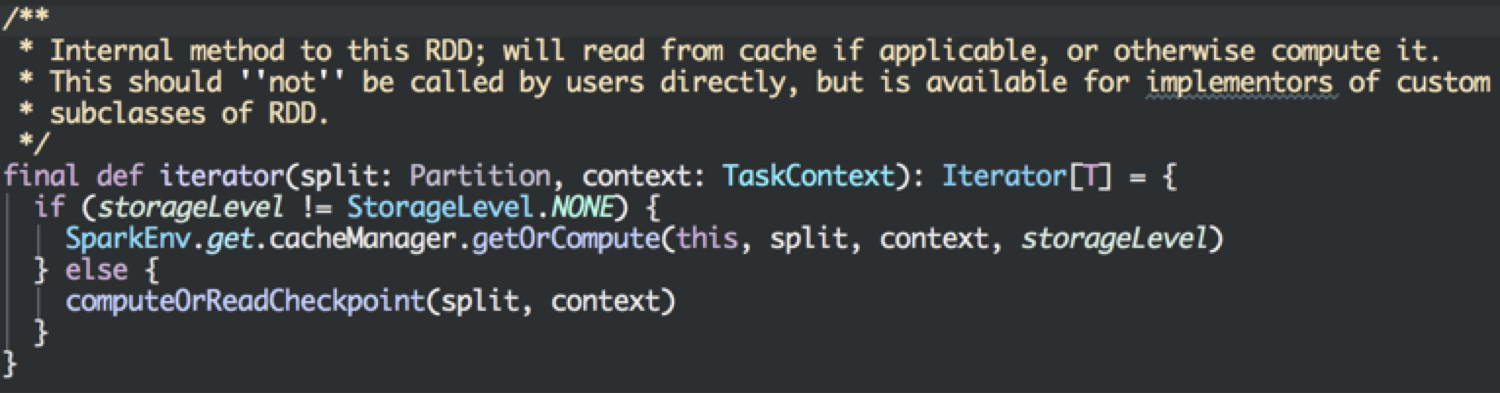
\includegraphics[scale=0.45]{./Figures/iterator_snippet}
	\end{figure}


\begin{itemize}
	\item {\bf Storage Levels}
	\begin{itemize}
		\item Disk
		\item Memory
		\item Off Heap (e.g. external memory stores like Tachyon)
		\item De-serialized
	\end{itemize}
\end{itemize}

}

%%%%%%%%%%%%%%%%%%%%%%%%%%%%%%%%%%%%%%%%%%%%%%%%%%%%%%%%%%
\frame {\frametitle{Making RDD from local collections}
%%%%%%%%%%%%%%%%%%%%%%%%%%%%%%%%%%%%%%%%%%%%%%%%%%%%%%%%%%
	\begin{itemize}
		\item {\bf Convert a local (on the driver) Seq[T] into RDD[T]}
	\end{itemize}

	\begin{figure}[h]
	\center
		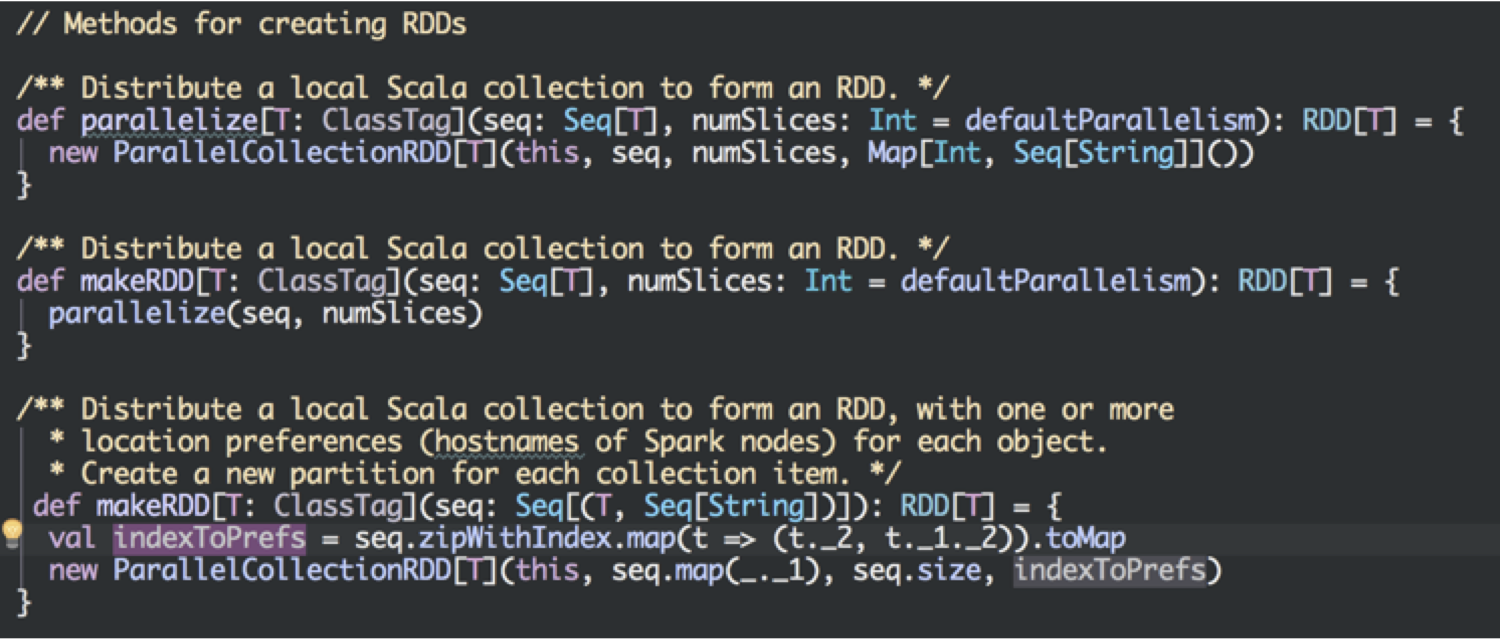
\includegraphics[scale=0.45]{./Figures/parallelize_snippet}
	\end{figure}


}

%%%%%%%%%%%%%%%%%%%%%%%%%%%%%%%%%%%%%%%%%%%%%%%%%%%%%%%%%%
\frame {\frametitle{Hadoop RDD Code Snippet}
%%%%%%%%%%%%%%%%%%%%%%%%%%%%%%%%%%%%%%%%%%%%%%%%%%%%%%%%%%
\begin{itemize}
	\item {\bf Reading HDFS data as <key, value> records}
\end{itemize}

\begin{figure}[h]
	\center
		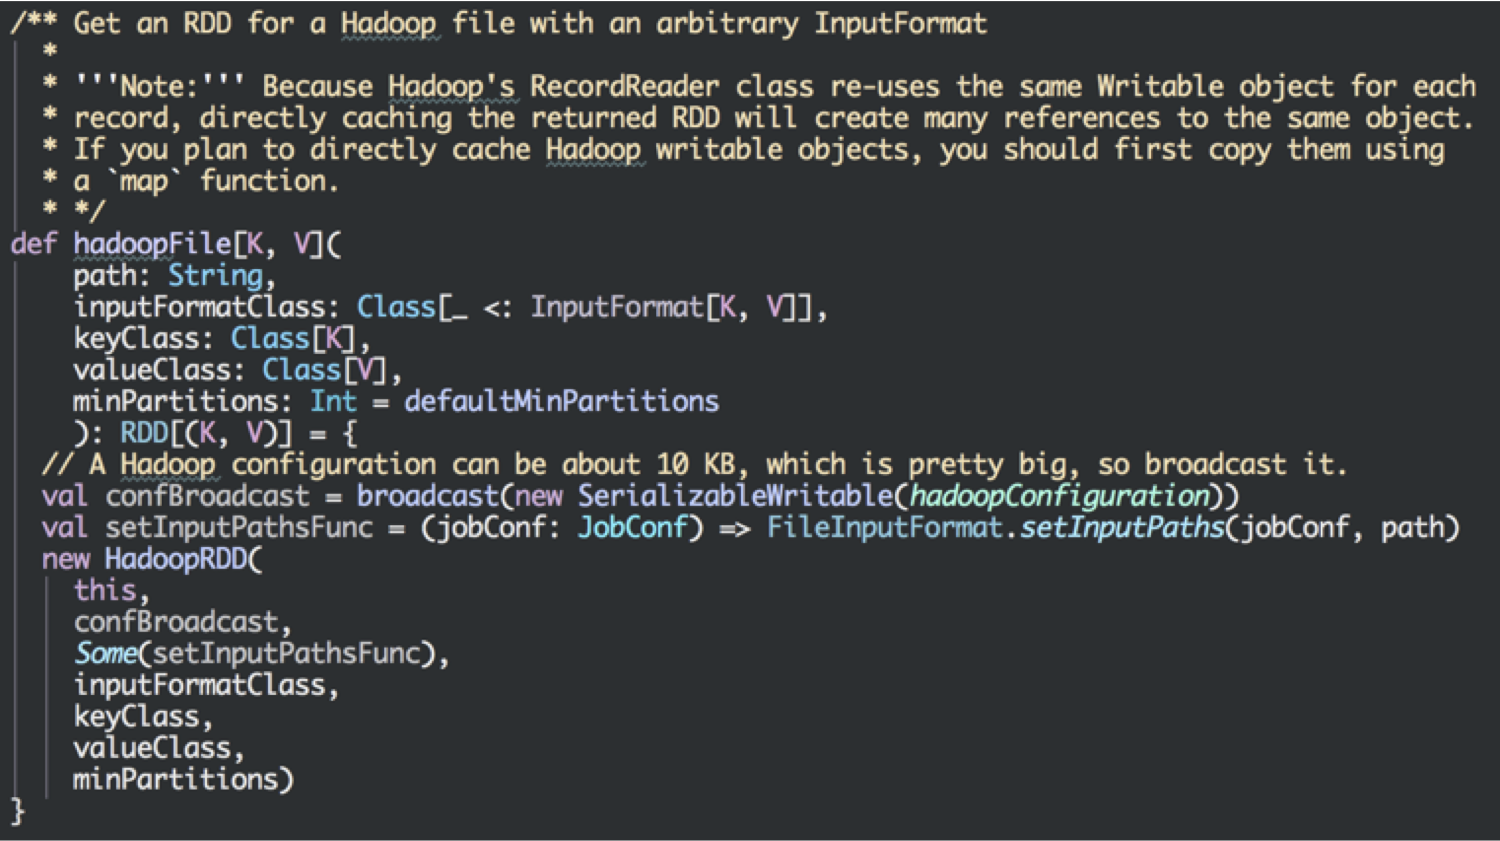
\includegraphics[scale=0.45]{./Figures/HadoopRDD_snippet}
\end{figure}
}

%%%%%%%%%%%%%%%%%%%%%%%%%%%%%%%%%%%%%%%%%%%%%%%%%%%%%%%%%%
\begin{frame}
%%%%%%%%%%%%%%%%%%%%%%%%%%%%%%%%%%%%%%%%%%%%%%%%%%%%%%%%%%
 \begin{colorblock}{blue}{lightblue}{ }
  \begin{center}
    \Large \textbf{\texttt{Understanding RDD Operations}}
  \end{center}
  \end{colorblock}
\end{frame}


%%%%%%%%%%%%%%%%%%%%%%%%%%%%%%%%%%%%%%%%%%%%%%%%%%%%%%%%%%
\frame {\frametitle{Common Transformations}
%%%%%%%%%%%%%%%%%%%%%%%%%%%%%%%%%%%%%%%%%%%%%%%%%%%%%%%%%%
\begin{columns}[t, onlytextwidth]
	\begin{column}[T]{.3\textwidth}
		\begin{center}
			\texttt{map(f: T => U)}	
		\end{center}
	\end{column}

	\begin{column}[T]{.5\textwidth}
		
			Returns a \texttt{MappedRDD[U]} by applying $f$ to each element
		
	\end{column}
\end{columns}

\begin{figure}[h]
	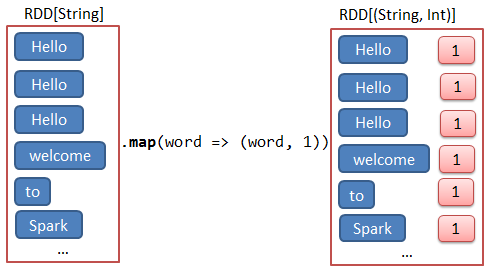
\includegraphics[scale=0.6]{./Figures/transformation_map}
\end{figure}

}

%%%%%%%%%%%%%%%%%%%%%%%%%%%%%%%%%%%%%%%%%%%%%%%%%%%%%%%%%%
\frame {\frametitle{Common Transformations}
%%%%%%%%%%%%%%%%%%%%%%%%%%%%%%%%%%%%%%%%%%%%%%%%%%%%%%%%%%
\begin{columns}[t, onlytextwidth]
	\begin{column}[T]{.4\textwidth}
		\begin{center}
			\texttt{flatMap(f: T => TraversableOnce[U])}	
		\end{center}
	\end{column}

	\begin{column}[T]{.4\textwidth}
		
			Returns a \texttt{FlatMappedRDD[U]} by first applying $f$ to each element, then flattening the results
		
	\end{column}
\end{columns}

\begin{figure}[h]
	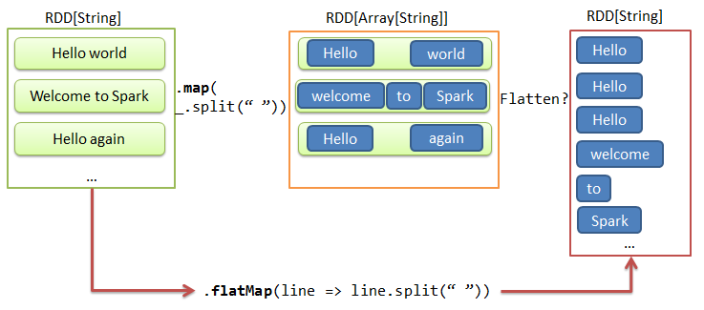
\includegraphics[scale=0.6]{./Figures/transformation_flatmap}
\end{figure}

}



%%%%%%%%%%%%%%%%%%%%%%%%%%%%%%%%%%%%%%%%%%%%%%%%%%%%%%%%%%

%%%%%%%%%%%%%%%%%%%%%%%%%%%%%%%%%%%%%%%%%%%%%%%%%%%%%%%%%%
\section{Spark Word Count}

\begin{frame}
 \begin{colorblock}{blue}{lightblue}{ }
  \begin{center}
    \Huge \textbf{\texttt{Detailed Example: Word Count}}
  \end{center}
  \end{colorblock}
\end{frame}

%%%%%%%%%%%%%%%%%%%%%%%%%%%%%%%%%%%%%%%%%%%%%%%%%%%%%%%%%%
\begin{frame}[fragile] 
\frametitle{Spark Word Count}
%%%%%%%%%%%%%%%%%%%%%%%%%%%%%%%%%%%%%%%%%%%%%%%%%%%%%%%%%%

\begin{itemize}
	\item Driver and \texttt{SparkContext}
	\begin{itemize}
		\item A SparkContext initializes the application driver, the latter then registers the application to the cluster manager, and gets a list of executors
		\item Then, the driver takes full control of the Spark job
	\end{itemize}
\end{itemize}

\begin{lstlisting}
	import org.apache.spark.SparkContext

	import org.apache.spark.SparkContext._

	val sc = new SparkContext("spark://...", "MyJob", "spark home", "additional jars") 
\end{lstlisting}

\end{frame}

%%%%%%%%%%%%%%%%%%%%%%%%%%%%%%%%%%%%%%%%%%%%%%%%%%%%%%%%%%
\begin{frame}[fragile] 
\frametitle{Spark Word Count}
%%%%%%%%%%%%%%%%%%%%%%%%%%%%%%%%%%%%%%%%%%%%%%%%%%%%%%%%%%
\begin{lstlisting}
	val lines = sc.textFile("input")
	val words = lines.flatMap(_.split(" ")) 
	val ones = words.map(_ -> 1)
	val counts = ones.reduceByKey(_ + _) 
	val result = counts.collectAsMap()
\end{lstlisting}

\begin{itemize}
	\item {\bf RDD lineage DAG is built on driver side with}
	\begin{itemize}
		\item Data source RDD(s)
		\item Transformation RDD(s), which are created by transformations
	\end{itemize}

	\vspace{10pt}

	\item Once an action is triggered on driver side, a job is submitted to the DAG scheduler of the driver
\end{itemize}

\end{frame}

%%%%%%%%%%%%%%%%%%%%%%%%%%%%%%%%%%%%%%%%%%%%%%%%%%%%%%%%%%

%%%%%%%%%%%%%%%%%%%%%%%%%%%%%%%%%%%%%%%%%%%%%%%%%%%%%%%%%%
\section{Caching and Storage}

\begin{frame}
 \begin{colorblock}{blue}{lightblue}{ }
  \begin{center}
    \Huge \textbf{\texttt{Caching and Storage}}
  \end{center}
  \end{colorblock}
\end{frame}

%%%%%%%%%%%%%%%%%%%%%%%%%%%%%%%%%%%%%%%%%%%%%%%%%%%%%%%%%%
\frame {\frametitle{Spark's Storage Module}
%%%%%%%%%%%%%%%%%%%%%%%%%%%%%%%%%%%%%%%%%%%%%%%%%%%%%%%%%%
\begin{itemize}
	\item {\bf The storage module}
	\begin{itemize}
		\item Access (I/O) ``external'' data sources: HDFS, Local Disk, RAM, remote data access through the network
		\item Caches RDDs using a variety of ``storage levels''
	\end{itemize}

	\vspace{20pt}

	\item {\bf Main components}
	\begin{itemize}
		\item The Cache Manager: uses the Block Manager to perform caching
		\item The Block Manager: distributed key/value store
	\end{itemize}
\end{itemize}
}

%%%%%%%%%%%%%%%%%%%%%%%%%%%%%%%%%%%%%%%%%%%%%%%%%%%%%%%%%%
\frame {\frametitle{Class Diagram of the Caching Component}
%%%%%%%%%%%%%%%%%%%%%%%%%%%%%%%%%%%%%%%%%%%%%%%%%%%%%%%%%%
\begin{figure}[h]
	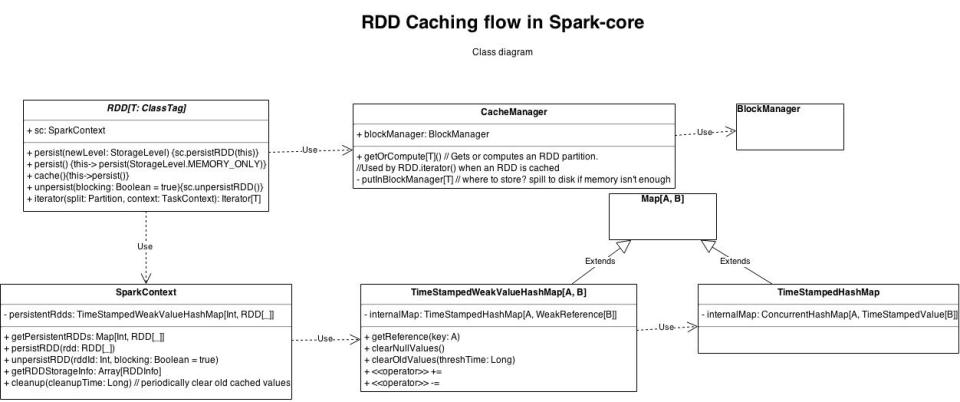
\includegraphics[scale=0.35]{./Figures/cache_classes}
\end{figure}
}

%%%%%%%%%%%%%%%%%%%%%%%%%%%%%%%%%%%%%%%%%%%%%%%%%%%%%%%%%%
\frame {\frametitle{How Caching Works}
%%%%%%%%%%%%%%%%%%%%%%%%%%%%%%%%%%%%%%%%%%%%%%%%%%%%%%%%%%
\begin{itemize}
	\item {\bf Frequently used RDD can be stored in memory}
	\begin{itemize}
		\item Deciding which RDD to cache is an art!
		\item One method, one short-cut: \texttt{persist()}, \texttt{cache()}
	\end{itemize}

	\vspace{20pt}

	\item {\bf \texttt{SparkContext} keeps track of cached RDD}
	\begin{itemize}
		\item Uses a data-structed called \texttt{persistentRDD}
		\item Maintains references to cached RDD, and eventually call the garbage collector
		\item Time-stamp based invalidation using \texttt{TimeStampedWeakValueHashMap[A, B]}
	\end{itemize}
\end{itemize}
}

%%%%%%%%%%%%%%%%%%%%%%%%%%%%%%%%%%%%%%%%%%%%%%%%%%%%%%%%%%
\frame {\frametitle{How Caching Works}
%%%%%%%%%%%%%%%%%%%%%%%%%%%%%%%%%%%%%%%%%%%%%%%%%%%%%%%%%%
\begin{columns}[t, onlytextwidth]
	\column[T]{.3\textwidth}
		
			\begin{figure}[h]
			  \centering
			  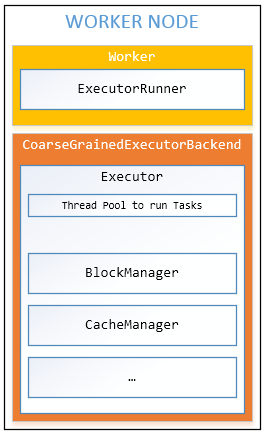
\includegraphics[scale=0.45]{./Figures/cache_workers}
			  \label{fig:spark_caching_workers}
			\end{figure}
	
	\column[T]{.6\textwidth}
		
			\begin{figure}[h]
			  \centering
			  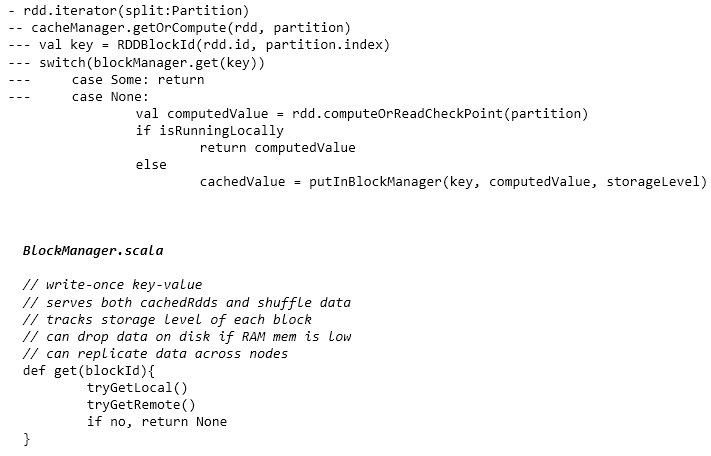
\includegraphics[scale=0.4]{./Figures/cache_stack}
			  \label{fig:caching_stack_calls}
			\end{figure}

\end{columns}
}

%%%%%%%%%%%%%%%%%%%%%%%%%%%%%%%%%%%%%%%%%%%%%%%%%%%%%%%%%%
\frame {\frametitle{The Block Manager}
%%%%%%%%%%%%%%%%%%%%%%%%%%%%%%%%%%%%%%%%%%%%%%%%%%%%%%%%%%
\begin{itemize}
	\item {\bf ``Write-once'' key-value store}
	\begin{itemize}
		\item One node per worker
		\item No updates, data is immutable
	\end{itemize}

	\vspace{20pt}

	\item {\bf Main tasks}
	\begin{itemize}
		\item Serves shuffle data (local or remote connections) and cached RDDs
		\item Tracks the ``Storage Level'' (RAM, disk) for each block
		\item Spills data to disk if memory is insufficient
		\item Handles data replication, if required
	\end{itemize}
\end{itemize}
}

%%%%%%%%%%%%%%%%%%%%%%%%%%%%%%%%%%%%%%%%%%%%%%%%%%%%%%%%%%
\frame {\frametitle{Storage Levels}
%%%%%%%%%%%%%%%%%%%%%%%%%%%%%%%%%%%%%%%%%%%%%%%%%%%%%%%%%%
\begin{itemize}
	\item {\bf The Block Manager can hold data in various storage tiers}
	\begin{itemize}
		\item \texttt{org.apache.spark.storage.StorageLevel} contains flags to indicate which tier to use
		\item Manual configuration, in the application
		\item Deciding the storage level to use for RDDs is not trivial
	\end{itemize}

	\vspace{10pt}

	\item {\bf Available storage tiers}
	\begin{itemize}
		\item RAM (default option): if the the RDD doesn't fit in memory, some partitions will not be cached (will be re-computed when needed)
		\item Tachyon (off java heap): reduces garbage collection overhead, the crash of an executor no longer leads to cached data loss
		\item Disk
	\end{itemize}

	\vspace{10pt}

	\item {\bf Data format}
	\begin{itemize}
		\item Serialized or as Java objects
		\item Replicated partitions
	\end{itemize}
\end{itemize}
}

%%%%%%%%%%%%%%%%%%%%%%%%%%%%%%%%%%%%%%%%%%%%%%%%%%%%%%%%%%

%%%%%%%%%%%%%%%%%%%%%%%%%%%%%%%%%%%%%%%%%%%%%%%%%%%%%%%%%%
\section{Resource Allocation}

\begin{frame}
 \begin{colorblock}{blue}{lightblue}{ }
  \begin{center}
    \Huge \textbf{\texttt{Resource Allocation: Spark Schedulers}}
  \end{center}
  \end{colorblock}
\end{frame}

%%%%%%%%%%%%%%%%%%%%%%%%%%%%%%%%%%%%%%%%%%%%%%%%%%%%%%%%%%
\frame {\frametitle{Spark Schedulers}
%%%%%%%%%%%%%%%%%%%%%%%%%%%%%%%%%%%%%%%%%%%%%%%%%%%%%%%%%%
\begin{itemize}
	\item {\bf Two main scheduler components, executed by the driver}
	\begin{itemize}
		\item The DAG scheduler
		\item The Task scheduler
	\end{itemize}

	\vspace{20pt}

	\item {\bf Objectives}
	\begin{itemize}
		\item Gain a broad understanding of how Spark submits Applications
		\item Understand how \textit{Stages} and \textit{Tasks} are built, and their optimization
		\item Understand interaction among various other Spark components
	\end{itemize}
\end{itemize}
}

%%%%%%%%%%%%%%%%%%%%%%%%%%%%%%%%%%%%%%%%%%%%%%%%%%%%%%%%%%
\frame {\frametitle{Submitting a Spark Application: A Walk Through}
%%%%%%%%%%%%%%%%%%%%%%%%%%%%%%%%%%%%%%%%%%%%%%%%%%%%%%%%%%
\begin{figure}[h]
  \centering
  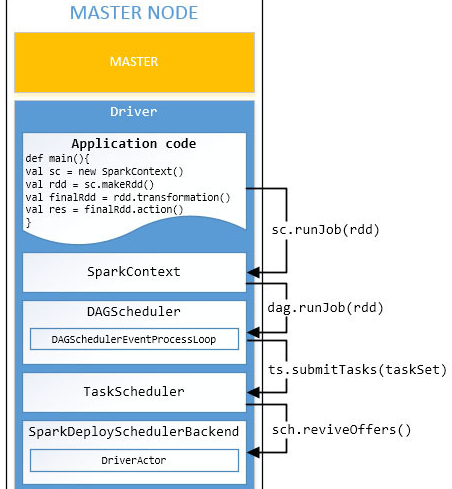
\includegraphics[scale=0.45]{./Figures/submit_modules}
  \label{fig:spark_submit_modules}
\end{figure}
}

%%%%%%%%%%%%%%%%%%%%%%%%%%%%%%%%%%%%%%%%%%%%%%%%%%%%%%%%%%
\frame {\frametitle{Submitting a Spark Application: Details}
%%%%%%%%%%%%%%%%%%%%%%%%%%%%%%%%%%%%%%%%%%%%%%%%%%%%%%%%%%
\begin{columns}[t, onlytextwidth]
	\column[T]{.5\textwidth}
		
			\begin{figure}[h]
			  \centering
			  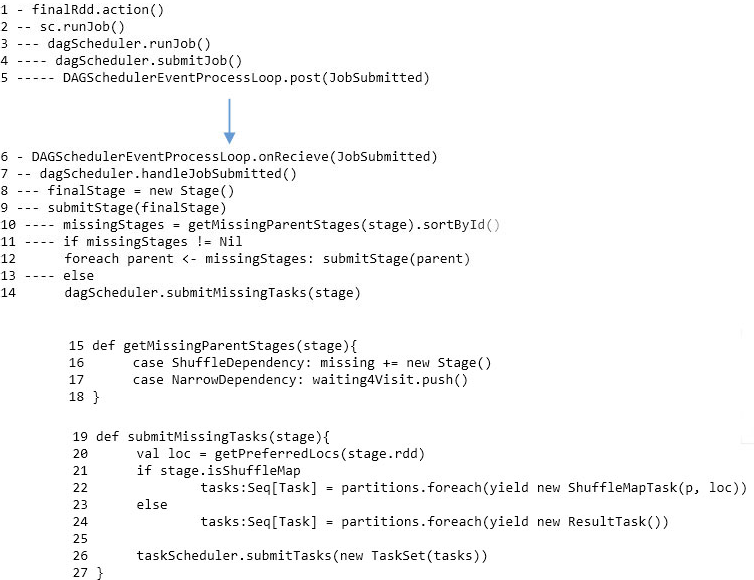
\includegraphics[scale=0.3]{./Figures/submit_stack_1}
			  \label{fig:spark_caching_workers}
			\end{figure}
	
	\column[T]{.5\textwidth}
		
			\begin{figure}[h]
			  \centering
			  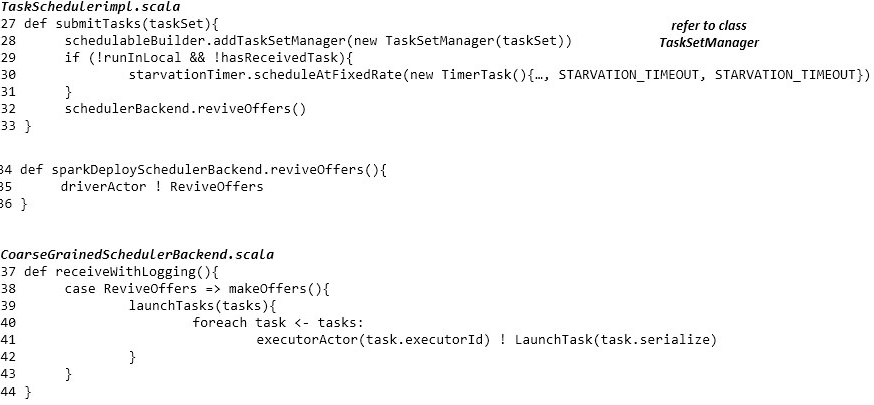
\includegraphics[scale=0.3]{./Figures/submit_stack_2}
			  \label{fig:caching_stack_calls}
			\end{figure}

\end{columns}
}

%%%%%%%%%%%%%%%%%%%%%%%%%%%%%%%%%%%%%%%%%%%%%%%%%%%%%%%%%%
\frame {\frametitle{The DAG Scheduler}
%%%%%%%%%%%%%%%%%%%%%%%%%%%%%%%%%%%%%%%%%%%%%%%%%%%%%%%%%%
\begin{itemize}
	\item {\bf Stage-oriented scheduling}
	\begin{itemize}
		\item Computes a DAG of stages for each job in the application
		\item[] \texttt{Lines 10-14}, details in \texttt{Lines 15-27}
		\item Keeps track of which RDD and stage output are materialized
		\item Determines an optimal schedule, minimizing stages
		\item Submit stages as sets of Tasks (\texttt{TaskSets}) to the Task scheduler
		\item[] \texttt{Line 26}
	\end{itemize}

	\item {\bf Data locality principle}
	\begin{itemize}
		\item Uses ``preferred location'' information (optionally) attached to each RDD
		\item[] \texttt{Line 20}
		\item Package this information into Tasks and send it to the Task scheduler
	\end{itemize}

	\item {\bf Manages Stage failures}
	\begin{itemize}
		\item Failure type: (intermediate) data loss of shuffle output files
		\item Failed stages will be resubmitted
		\item NOTE: Task failures are handled by the Task scheduler, which simply resubmit them if they can be computed with no dependency on previous output
	\end{itemize}

\end{itemize}
}

%%%%%%%%%%%%%%%%%%%%%%%%%%%%%%%%%%%%%%%%%%%%%%%%%%%%%%%%%%
\frame {\frametitle{The DAG Scheduler: Implementation Details}
%%%%%%%%%%%%%%%%%%%%%%%%%%%%%%%%%%%%%%%%%%%%%%%%%%%%%%%%%%
\begin{itemize}
	\item {\bf Implemented as an event queue}
	\begin{itemize}
		\item Uses a daemon thread to handle various kinds of events
		\item[] \texttt{Line 6}
		\item \texttt{JobSubmitted}, \texttt{JobCancelled}, \texttt{CompletionEvent}
		\item The thread ``swipes'' the queue, and routes event to the corresponding handlers
	\end{itemize}

	\vspace{10pt}

	\item {\bf What happens when a job is submitted to the DAGScheduler?}
	\begin{itemize}
		\item \texttt{JobWaiter} object is created
		\item \texttt{JobSubmitted} event is fired
		\item The daemon thread blocks and wait for a job result
		\item[] \texttt{Lines 3,4}
	\end{itemize}

\end{itemize}
}

%%%%%%%%%%%%%%%%%%%%%%%%%%%%%%%%%%%%%%%%%%%%%%%%%%%%%%%%%%
\frame {\frametitle{The DAG Scheduler: Implementation Details (2)}
%%%%%%%%%%%%%%%%%%%%%%%%%%%%%%%%%%%%%%%%%%%%%%%%%%%%%%%%%%
\begin{itemize}
	\item {\bf Who handles the \texttt{JobSubmitted} event?}
	\begin{itemize}
		\item Specific handler called \texttt{handleJobSubmitted}
		\item[] \texttt{Line 6}
	\end{itemize}


	\item {\bf Walk-through to the Job Submitted handler}
	\begin{itemize}
		\item Create a new job, called \texttt{ActiveJob}
		\item New job starts with only 1 stage, corresponding to the last stage of the job upon which an action is called
		\item[] \texttt{Lines 8-9}
		\item Use the dependency information to produce additional stages
		\begin{itemize}
			\item Shuffle Dependency: create a new map stage
			\item[] \texttt{Line 16}
			\item Narrow Dependency: pipes them into a single stage
			\item[] \texttt{getMissingParentStages}
		\end{itemize}
	\end{itemize}
\end{itemize}
}

%%%%%%%%%%%%%%%%%%%%%%%%%%%%%%%%%%%%%%%%%%%%%%%%%%%%%%%%%%
\frame {\frametitle{More About Stages}
%%%%%%%%%%%%%%%%%%%%%%%%%%%%%%%%%%%%%%%%%%%%%%%%%%%%%%%%%%
\begin{itemize}
	\item {\bf What is a DAG}
	\begin{itemize}
		\item Directed acyclic graph of stages
		\item Stage boundaries determined by the shuffle phase
		\item Stages are run in \emph{topological order}
	\end{itemize}

	\item {\bf Definition of a Stage}
	\begin{itemize}
		\item Set of \emph{independent} tasks
		\item All tasks of a stage apply the same function
		\item All tasks of a stage have the same dependency type
		\item All tasks in a stage belong to a \texttt{TaskSet}
	\end{itemize}

	\item {\bf Stage types}
	\begin{itemize}
		\item Shuffle Map Stage: stage tasks results are inputs for another stage
		\item Result Stage: tasks compute the final action that initiated a job (e.g., \texttt{count()}, \texttt{save()}, etc.)
	\end{itemize}

\end{itemize}
}

%%%%%%%%%%%%%%%%%%%%%%%%%%%%%%%%%%%%%%%%%%%%%%%%%%%%%%%%%%
\frame {\frametitle{The Task Scheduler}
%%%%%%%%%%%%%%%%%%%%%%%%%%%%%%%%%%%%%%%%%%%%%%%%%%%%%%%%%%
\begin{itemize}
	\item {\bf Task oriented scheduling}
	\begin{itemize}
		\item Schedules tasks for a \emph{single} \texttt{SparkContext}
		\item Submits tasks sets produced by the DAG Scheduler
		\item Retries failed tasks
		\item Takes care of \emph{stragglers} with speculative execution
		\item Produces events for the DAG Scheduler
	\end{itemize}

	\item {\bf Implementation details}
	\begin{itemize}
		\item The Task scheduler creates a \texttt{TaskSetManager} to wrap the \texttt{TaskSet} from the DAG scheduler
		\item[] \texttt{Line 28}
		\item The \texttt{TaskSetManager} class operates as follows:
		\begin{itemize}
			\item Keeps track of each task status
			\item Retries failed tasks
			\item Imposes data locality using \emph{delayed scheduling}
			\item[] \texttt{Lines 29,30}
		\end{itemize}
		\item Message passing implemented using \emph{Actors}, and precisely using the \emph{Akka framework}
	\end{itemize}
\end{itemize}
}

%%%%%%%%%%%%%%%%%%%%%%%%%%%%%%%%%%%%%%%%%%%%%%%%%%%%%%%%%%
\frame {\frametitle{Running Tasks on Executors}
%%%%%%%%%%%%%%%%%%%%%%%%%%%%%%%%%%%%%%%%%%%%%%%%%%%%%%%%%%
\begin{columns}[t, onlytextwidth]
	\column[T]{.5\textwidth}
		
			\begin{figure}[h]
			  \centering
			  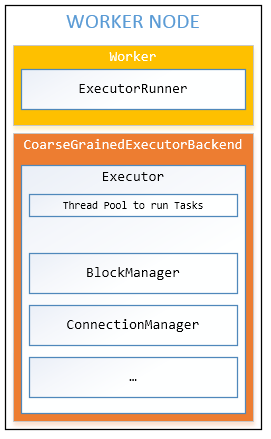
\includegraphics[scale=0.5]{./Figures/executor_components}
			  \label{fig:spark_caching_workers}
			\end{figure}
	
	\column[T]{.5\textwidth}
		
			\begin{figure}[h]
			  \centering
			  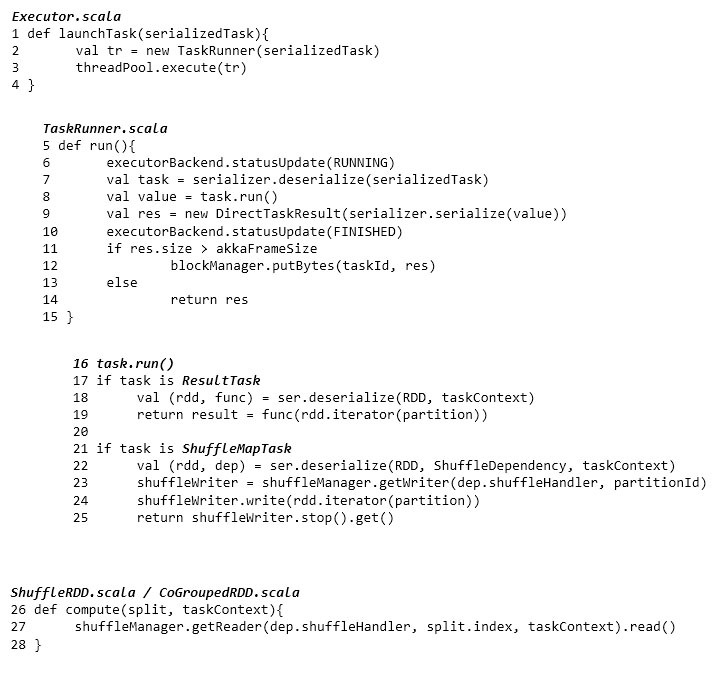
\includegraphics[scale=0.4]{./Figures/executor_stack}
			  \label{fig:caching_stack_calls}
			\end{figure}

\end{columns}
}

%%%%%%%%%%%%%%%%%%%%%%%%%%%%%%%%%%%%%%%%%%%%%%%%%%%%%%%%%%
\frame {\frametitle{Running Tasks on Executors}
%%%%%%%%%%%%%%%%%%%%%%%%%%%%%%%%%%%%%%%%%%%%%%%%%%%%%%%%%%
\begin{itemize}
	\item {\bf Executors run two kinds of tasks}
	\begin{itemize}
		\item \texttt{ResultTask}: apply the action on the RDD, once it has been computed, alongside all its dependencies
		\item[] \texttt{Line 19}
		\item \texttt{ShuffleTask}: use the Block Manager to store shuffle output using the \texttt{ShuffleWriter}
		\item[] \texttt{Lines 23,24}
		\item The \texttt{ShuffleRead} component depends on the type of the RDD, which is determined by the compute function and the transformation applied to it
	\end{itemize}
\end{itemize}
}

%%%%%%%%%%%%%%%%%%%%%%%%%%%%%%%%%%%%%%%%%%%%%%%%%%%%%%%%%%


%%%%%%%%%%%%%%%%%%%%%%%%%%%%%%%%%%%%%%%%%%%%%%%%%%%%%%%%%%
\section{Data Shuffling}

\begin{frame}
 \begin{colorblock}{blue}{lightblue}{ }
  \begin{center}
    \Huge \textbf{\texttt{Data Shuffling}}
  \end{center}
  \end{colorblock}
\end{frame}

%%%%%%%%%%%%%%%%%%%%%%%%%%%%%%%%%%%%%%%%%%%%%%%%%%%%%%%%%%
\frame {\frametitle{The Spark Shuffle Mechanism}
%%%%%%%%%%%%%%%%%%%%%%%%%%%%%%%%%%%%%%%%%%%%%%%%%%%%%%%%%%
\begin{itemize}
	\item {\bf Same concept as for Hadoop MapReduce, involving:}
	\begin{itemize}
		\item Storage of ``intermediate'' results on the local file-system
		\item Partitioning of ``intermediate'' data
		\item Serialization / De-serialization
		\item Pulling data over the network
	\end{itemize}

	\vspace{20pt}

	\item {\bf Transformations requiring a shuffle phase}
	\begin{itemize}
		\item \texttt{groupByKey()}, \texttt{reduceByKey()}, \texttt{sortByKey()}, \texttt{distinct()}
	\end{itemize}

	\vspace{20pt}

	\item {\bf Various types of Shuffle}
	\begin{itemize}
		\item \emph{Hash Shuffle}
		\item \emph{Consolidate Hash Shuffle}
		\item \emph{Sort-based Shuffle}
	\end{itemize}
\end{itemize}
}

%%%%%%%%%%%%%%%%%%%%%%%%%%%%%%%%%%%%%%%%%%%%%%%%%%%%%%%%%%
\frame {\frametitle{The Spark Shuffle Mechanism: an Illustration}
%%%%%%%%%%%%%%%%%%%%%%%%%%%%%%%%%%%%%%%%%%%%%%%%%%%%%%%%%%
\begin{figure}[h]
  \centering
  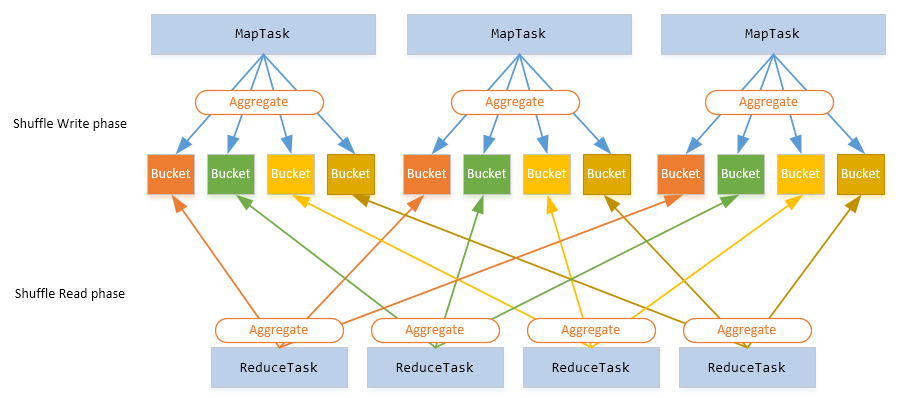
\includegraphics[scale=0.35]{./Figures/spark_shuffle}
  \label{fig:spark_shuffle}
\end{figure}

\begin{itemize}
	\item {\bf Data Aggregation}
	\begin{itemize}
		\item Defined on \texttt{ShuffleMapTask}
		\item Two methods available:
		\begin{itemize}
			\item \texttt{AppendOnlyMap}: in-memory hash table combiner
			\item \texttt{ExternalAppendOnlyMap}: memory + disk hash table combiner
		\end{itemize}
	\end{itemize}
	\item {\bf Batching disk writes to increase throughput}
\end{itemize}
}

%%%%%%%%%%%%%%%%%%%%%%%%%%%%%%%%%%%%%%%%%%%%%%%%%%%%%%%%%%
\frame {\frametitle{The Spark Shuffle Mechanism: Implementation Details}
%%%%%%%%%%%%%%%%%%%%%%%%%%%%%%%%%%%%%%%%%%%%%%%%%%%%%%%%%%
\begin{figure}[h]
  \centering
  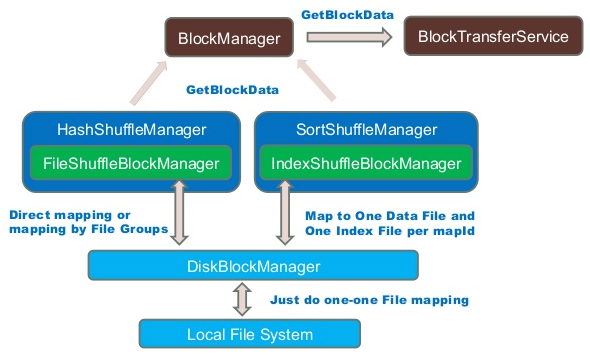
\includegraphics[scale=0.33]{./Figures/shuffle_diagram}
  \label{fig:spark_shuffle_diagram}
\end{figure}

\begin{itemize}
	\item {\bf Pluggable component}
	\begin{itemize}
		\item \emph{Shuffle Manager}: components registered to \texttt{SparkEnv}, configured through \texttt{SparkConf}
		\item \emph{Shuffle Writer}: tracks ``intermediate data'' for the \texttt{MapOutputTracker}
		\item \emph{Shuffle Reader}: pull-based mechanism used by the \texttt{ShuffleRDD}
		\item \emph{Shuffle Block Manager}: mapping between logical partitioning and the physical layout of data
	\end{itemize}
\end{itemize}
}

%%%%%%%%%%%%%%%%%%%%%%%%%%%%%%%%%%%%%%%%%%%%%%%%%%%%%%%%%%
\frame {\frametitle{The Hash Shuffle Mechanism}
%%%%%%%%%%%%%%%%%%%%%%%%%%%%%%%%%%%%%%%%%%%%%%%%%%%%%%%%%%
\begin{figure}[h]
  \centering
  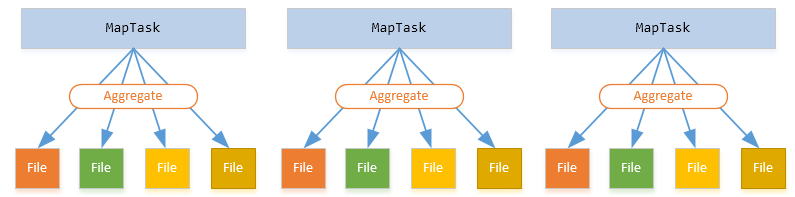
\includegraphics[scale=0.35]{./Figures/spark_shuffle_hash}
  \label{fig:spark_shuffle_hash}
\end{figure}

\begin{itemize}
	\item {\bf Map Tasks write output to multiple files}
	\begin{itemize}
		\item Assume: $m$ map tasks and $r$ reduce tasks
		\item Then: $m \times r$ shuffle files as well as in-memory buffers (for batching writes)
	\end{itemize}

	\item {\bf Be careful on storage space requirements!}
	\begin{itemize}
		\item Buffer size must not be too big with many tasks
		\item Buffer size must not be too small, for otherwise throughput decreases
	\end{itemize}
\end{itemize}
}

%%%%%%%%%%%%%%%%%%%%%%%%%%%%%%%%%%%%%%%%%%%%%%%%%%%%%%%%%%
\frame {\frametitle{The Consolidate Hash Shuffle Mechanism}
%%%%%%%%%%%%%%%%%%%%%%%%%%%%%%%%%%%%%%%%%%%%%%%%%%%%%%%%%%
\begin{figure}[h]
  \centering
  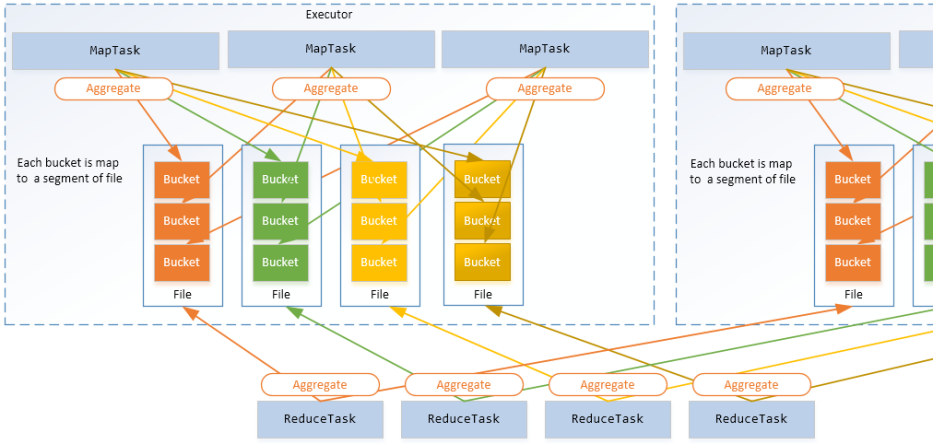
\includegraphics[scale=0.35]{./Figures/spark_shuffle_consolidate}
  \label{fig:spark_shuffle_consolidate}
\end{figure}

\begin{itemize}
	\item {\bf Addresses buffer size problems}
	\begin{itemize}
		\item Executor view vs. Task view
		\item Buckets are consolidated in a single file
		\item Hence: $F = C \times r$ files and buffers, where $C$ is the number of Task threads within an Executor
	\end{itemize}

\end{itemize}
}

%%%%%%%%%%%%%%%%%%%%%%%%%%%%%%%%%%%%%%%%%%%%%%%%%%%%%%%%%%
\frame {\frametitle{The Sort-based Shuffle Mechanism}
%%%%%%%%%%%%%%%%%%%%%%%%%%%%%%%%%%%%%%%%%%%%%%%%%%%%%%%%%%
\begin{figure}[h]
  \centering
  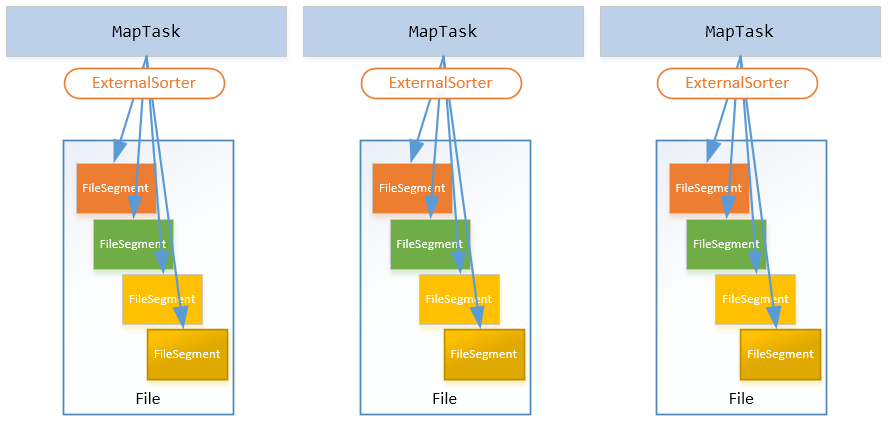
\includegraphics[scale=0.35]{./Figures/spark_shuffle_sort}
  \label{fig:spark_shuffle_sort}
\end{figure}

\begin{itemize}
	\item {\bf Implements the Hadoop Shuffle mechanism}
	\begin{itemize}
		\item Single shuffle file, plus an index file to find ``buckets''
		\item Very beneficial for write throughput, as more disk writes can be batched
	\end{itemize}

	\item {\bf Sorting mechanism}
	\begin{itemize}
		\item Pluggable external sorter
		\item Degenerates to Hash Shuffle if no sorting is required
	\end{itemize}

\end{itemize}
}

%%%%%%%%%%%%%%%%%%%%%%%%%%%%%%%%%%%%%%%%%%%%%%%%%%%%%%%%%%
\frame {\frametitle{Data Transfer: Implementation Details}
%%%%%%%%%%%%%%%%%%%%%%%%%%%%%%%%%%%%%%%%%%%%%%%%%%%%%%%%%%
\begin{itemize}
	\item {\bf BlockTransfer Service}
	\begin{itemize}
		\item General interface for \texttt{ShuffleFetcher}
		\item Uses \texttt{BlockDataManager} to get local data
	\end{itemize}

	\vspace{10pt}

	\item {\bf Shuffle Client}
	\begin{itemize}
		\item Manages and wraps the ``client-side'', setting up the \texttt{TransportContext} and \texttt{TransportClient}
	\end{itemize}
	
	\vspace{10pt}

	\item {\bf Transport Context}: manages the transport layer
	\item {\bf Transport Server}: streaming server
	\item {\bf Transport Client}: fetches consecutive chunks
\end{itemize}
}

%%%%%%%%%%%%%%%%%%%%%%%%%%%%%%%%%%%%%%%%%%%%%%%%%%%%%%%%%%
\frame {\frametitle{Data Transfer: an Illustration}
%%%%%%%%%%%%%%%%%%%%%%%%%%%%%%%%%%%%%%%%%%%%%%%%%%%%%%%%%%
\begin{figure}[h]
  \centering
  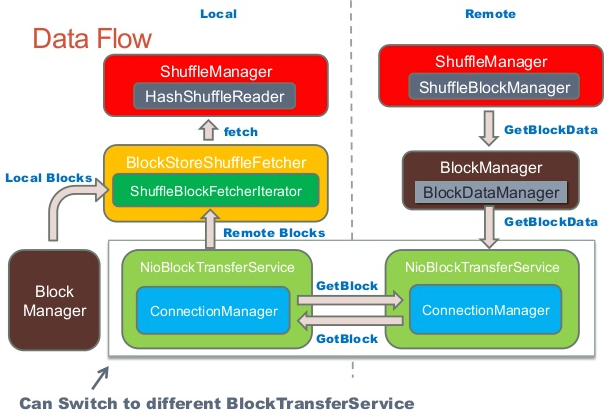
\includegraphics[scale=0.35]{./Figures/shuffle_data_transfer}
  \label{fig:spark_shuffle_sort}
\end{figure}
}

%%%%%%%%%%%%%%%%%%%%%%%%%%%%%%%%%%%%%%%%%%%%%%%%%%%%%%%%%%


%%%%%%%%%%%%%%%%%%%%%%%%%%%%%%%%%%%%%%%%%%%%%%%%%%%%%%%%%%
\section{Spark Tuning}

\begin{frame}
 \begin{colorblock}{blue}{lightblue}{ }
  \begin{center}
    \Huge \textbf{\texttt{Spark Tuning with a Running Example}}
  \end{center}
  \end{colorblock}
\end{frame}

% \input{./tuning.tex}
%%%%%%%%%%%%%%%%%%%%%%%%%%%%%%%%%%%%%%%%%%%%%%%%%%%%%%%%%%

\end{document}
